\documentclass{beamer}
\usetheme{focus}

\usepackage{amsmath}
\usepackage{braket}
\usepackage{listing}

\definecolor{main}{RGB}{170, 85, 0}
\definecolor{background}{RGB}{240, 247, 255}

\title{Implementazione di un algoritmo KNN multiclasse su hardware quantistico}
\subtitle{Tesi di laurea sperimentale in fisica}
\author{Mariano Mollo N85000880\texorpdfstring{\\}{,} Relatori: \texorpdfstring{\\}{,} Giovanni Acampora \texorpdfstring{\\}{,} Autilia Vitiello}
\titlegraphic{
\includegraphics[scale=0.15]{gfx/logo-federico-II-blu}}
\institute{Università degli Studi di Napoli Federico II\texorpdfstring{\\}{,} Scuola Politecnica e delle Scienze di Base}
\date{ottobre 2019}

% [ ] Le icone sono sgranate, sostiuirle con versioni di qualità migliore. 
% [ ] Mettere slide sulle porte quantistiche usate
% [x] Si può inserire un'altra slide in cui si scrive l'equazione del QDB. 
% [x] Quando si introducono i qubit, mettere una slide sui registri a qubit multipli. 
% [x] Mettere gli obiettivi appena dopo l'introduzione. 

\begin{document}
    \begin{frame}
        \maketitle
    \end{frame}

    \section{Introduzione}

    \begin{frame}{Machine learning}
        \begin{columns}
            \column{0.3\textwidth}
            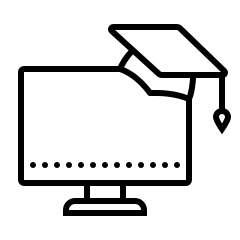
\includegraphics[width=\textwidth]{gfx/icons/icons8-machine-learning-240.png}
            Il machine learning permette ai computer di imparare dai dati
            \column{0.7\textwidth}
            Gli algoritmi di ML prevedono spesso di
            \begin{itemize}
                \item risolvere grandi sistemi di equazioni lineari
                \item invertire grandi matrici
                \item calcolare distanze
            \end{itemize}
            Effettuare questi calcoli su insiemi dati grandi e complessi diventa difficile
        \end{columns}
    \end{frame}

    \begin{frame}{Quantum computing}
        \begin{columns}
            \column{0.3\textwidth}
            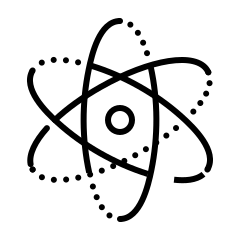
\includegraphics[width=\textwidth]{gfx/icons/icons8-physics-240.png}
            Il quantum computing studia la costruzione e l'uso di hardware di elaborazione basato sulla meccanica quantistica
            \column{0.7\textwidth}
            \begin{itemize}
                \item Il quantum computing lavora con vettori in spazi di Hilbert complessi
                \item I computer quantistici eseguono operazioni lineari sui qubit
                \item Sistemi a molti qubit sono descritti da grandi vettori che possono essere manipolati in parallelo
                \item Il machine learning prevede la manipolazione di grandi vettori e matrici
            \end{itemize}
        \end{columns}
    \end{frame}

    \begin{frame}{Quantum machine learning}
        \begin{columns}
            \column{0.3\textwidth}
            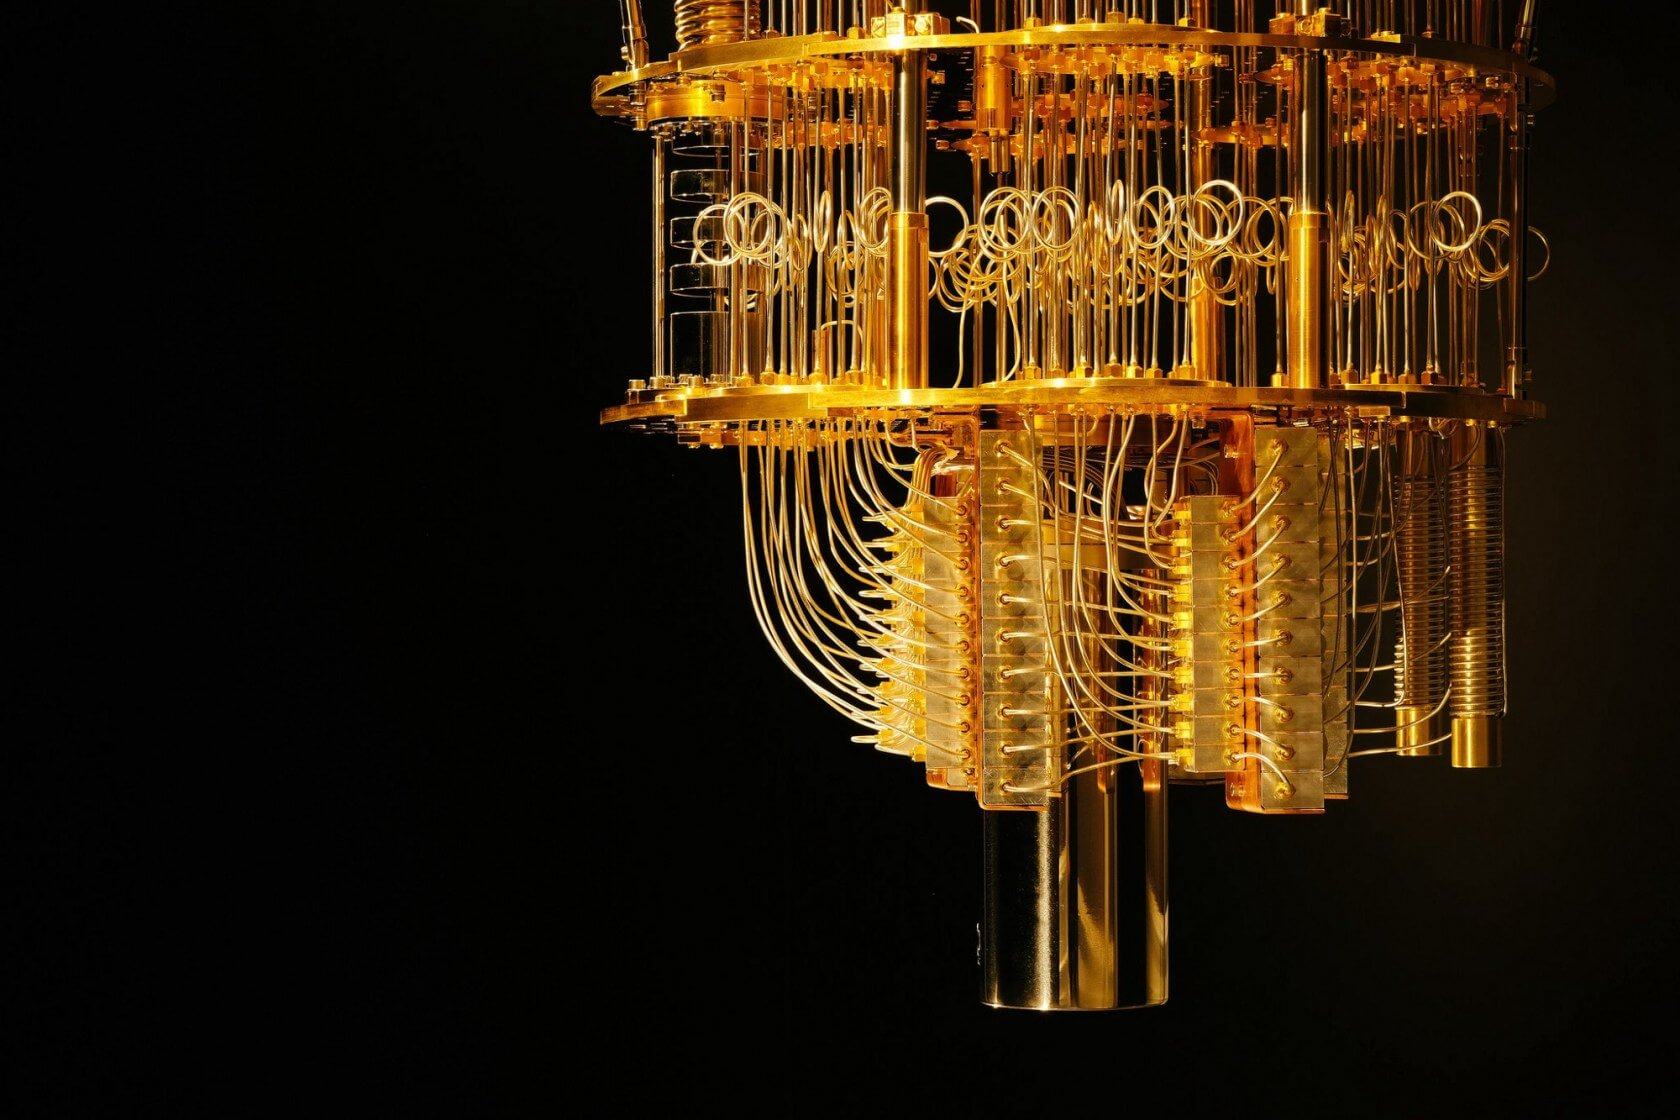
\includegraphics[width=\textwidth]{gfx/quantum-computer.jpg}
            \column{0.7\textwidth}
            L'uso dei computer quantistici per risolvere problemi classici difficili o classi di problemi completamente nuove è chiamato machine learning quantistico, 
            ovvero permettere ai computer quantistici di imparare dai dati più velocemente dei computer classici
        \end{columns}
    \end{frame}

    \begin{frame}{Domanda di ricerca}
        È possibile implementare su un computer quantistico un 
        algoritmo k-nearest neighbours multiclasse, in modo da 
        migliorare le prestazioni ed il numero di problemi risolvibili? 
    \end{frame}

    \begin{frame}{Obiettivi}
        \begin{itemize}
            \item Riprodurre l'algoritmo di classificazione binaria KNN quantistico proposto da Schuld et al. 
            \item Implementarne una versione multiclasse
            \item Analizzare le capacità dell'algoritmo usando l'hardware quantistico attualmente disponibile
            \item Analizzare esperimenti più complessi tramite simulazione
        \end{itemize}
    \end{frame}

    \section{Machine learning}

    \begin{frame}{Machine learning}
        \begin{columns}
            \column{.5\textwidth}
            Il machine learning è un ramo dell'intelligenza artificiale che permette ai computer di apprendere dai dati. 

            L'apprendimento può formalizzarsi attraverso la definizione di modelli matematici, usati per
            \column{.5\textwidth}
            \begin{itemize}
                \item effettuare previsioni (apprendimento supervisionato)
                \item trovare regolarità in processi complessi (apprendimento non supervisionato)
                \item effettuare scelte per ottenere un risultato ottimale (apprendimento per rinforzo)
            \end{itemize}
        \end{columns}
    \end{frame}

    \begin{frame}{Machine learning supervisionato}
        \begin{block}{Definizione del problema}
            Dato un insieme dati in input con i corrispondenti output, predire l'output di un nuovo input ignoto. 
        \end{block}
        \begin{tabular}{cc}
            Input & Output \\ \hline
            facce & emozioni \\ 
            battito cardiaco & stato di salute \\ 
            meteo dell'anno scorso & meteo di domani \\ 
            messaggio di un utente & intenzione del messaggio \\ 
            cronologia di ricerca & probabilità di cliccare su un annuncio
        \end{tabular}
    \end{frame}

    \begin{frame}{k-nearest neighbours classico}
        L'algoritmo KNN è uno tra i più semplici del ML ed è un lazy learner
        \begin{columns}
            \column{0.3\textwidth}
            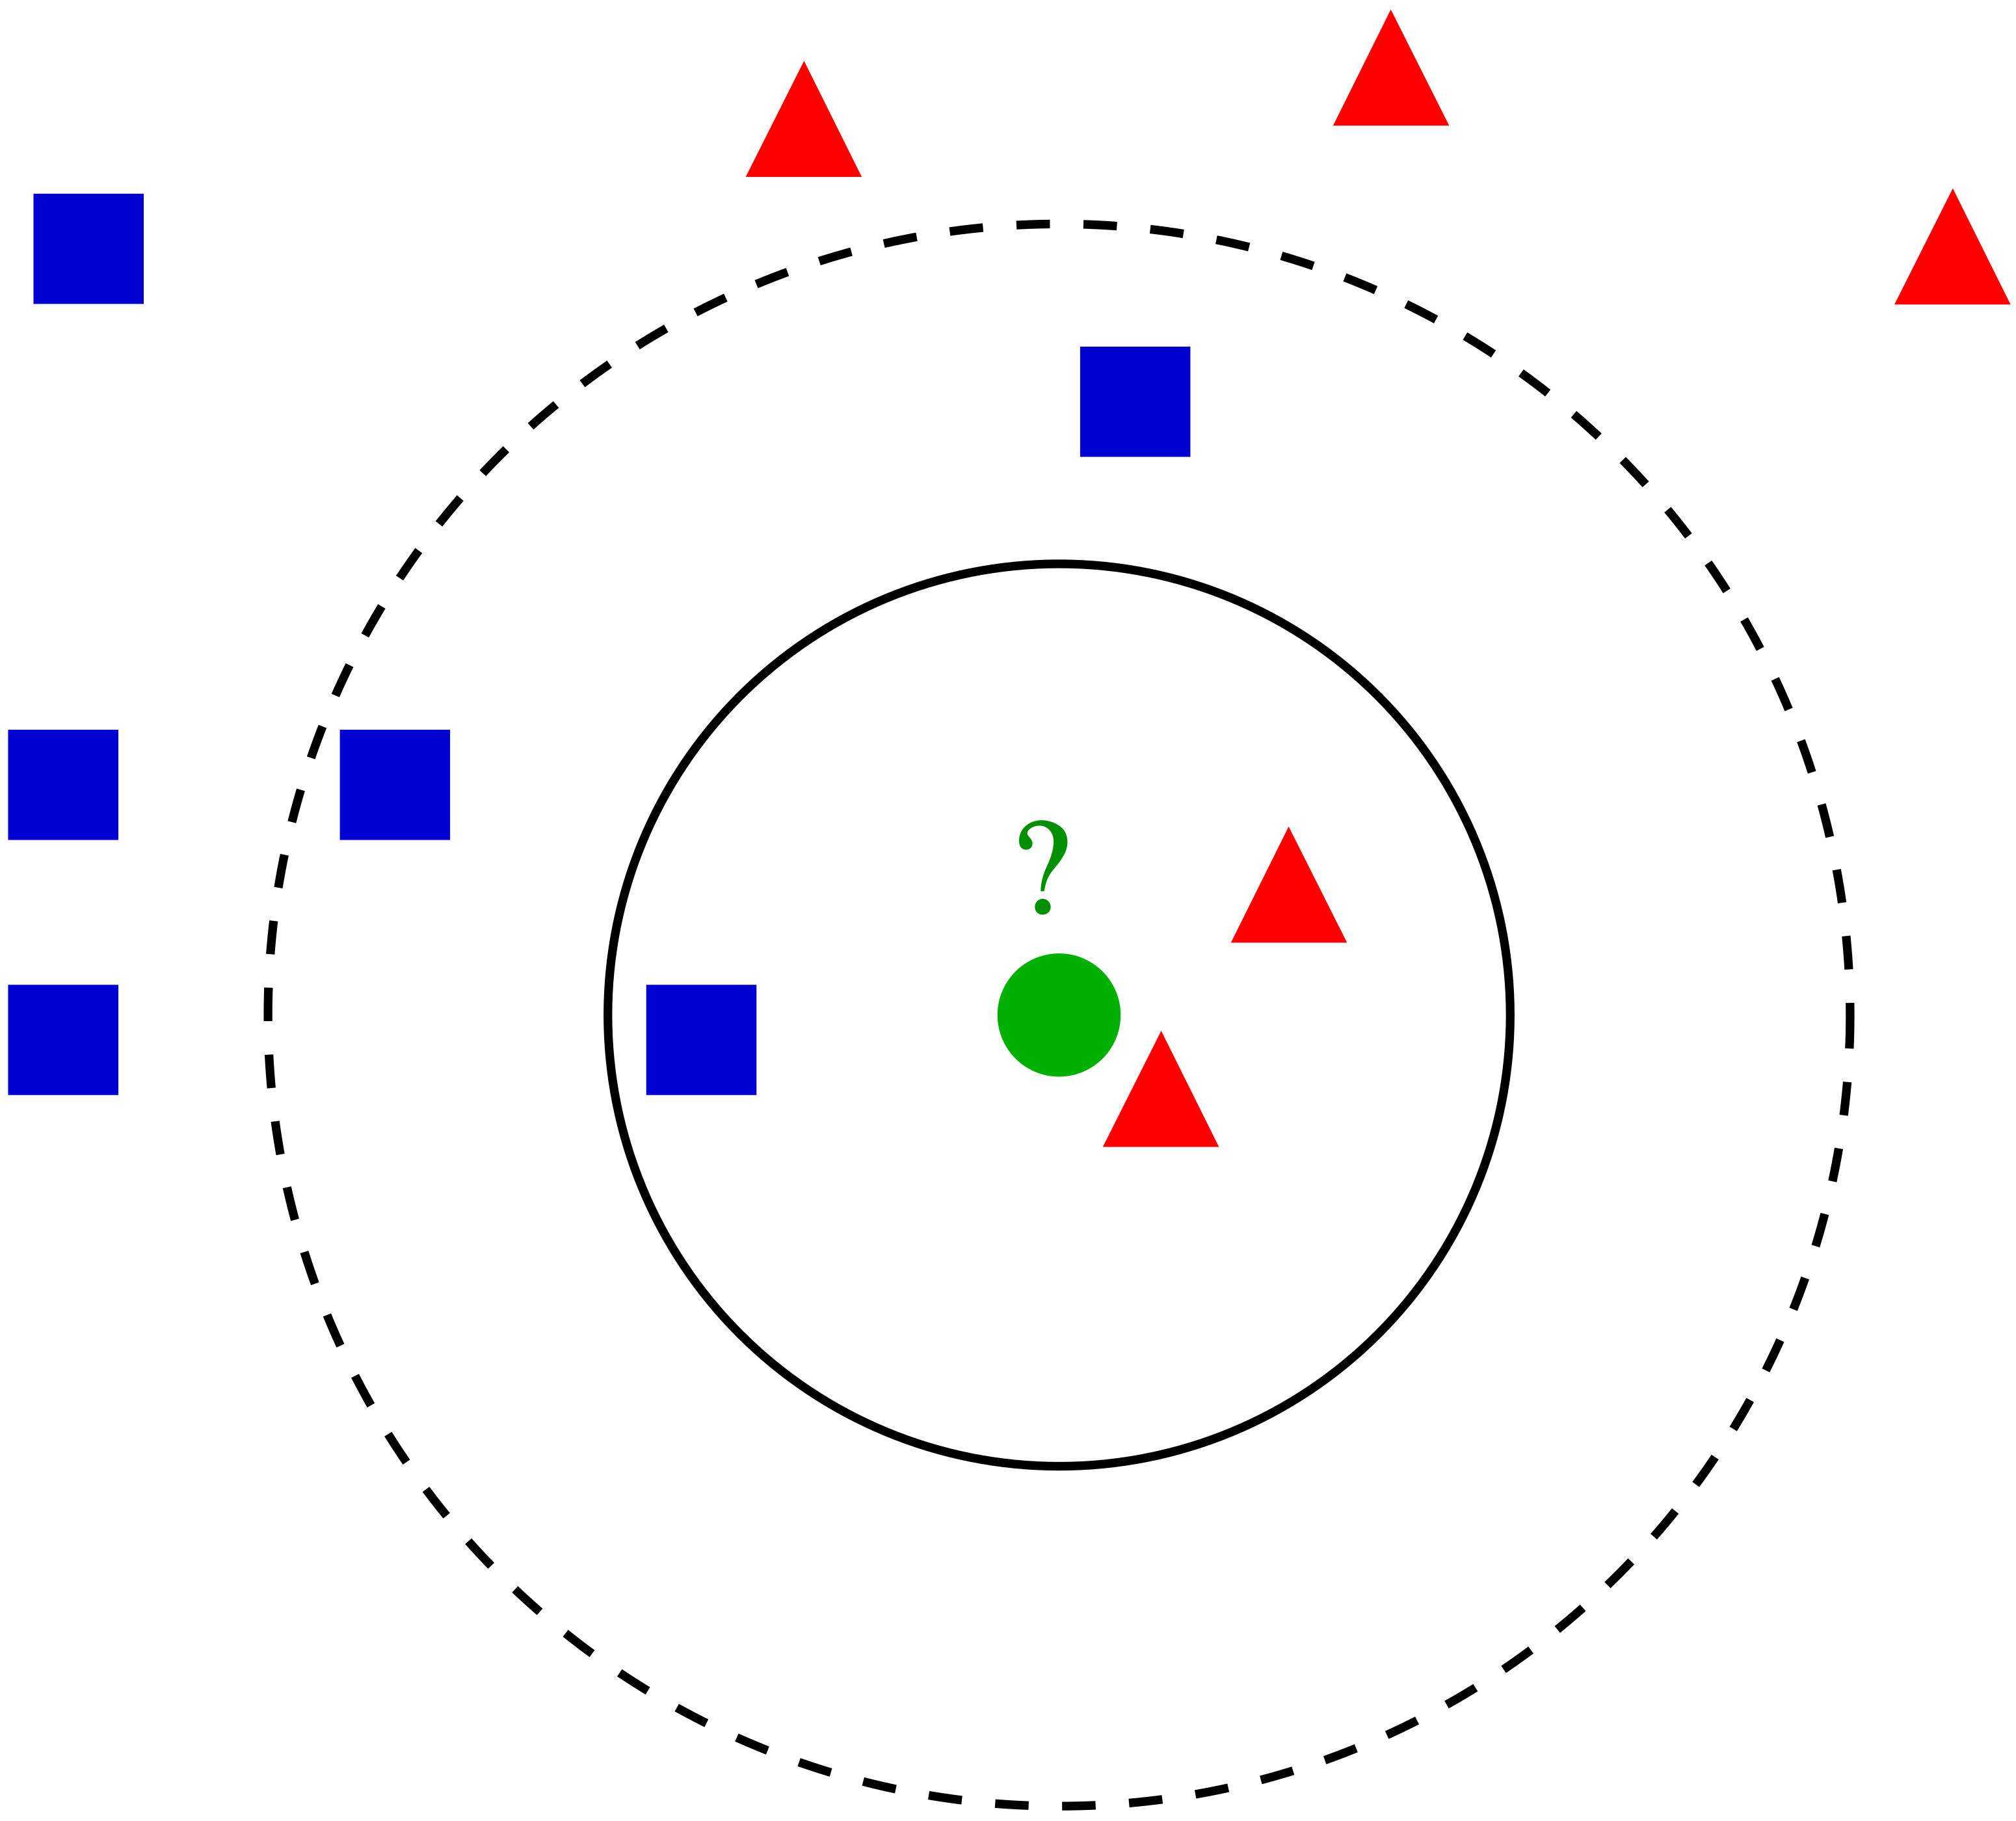
\includegraphics[width=\textwidth]{gfx/KnnClassification.png}
            \column{0.7\textwidth}
            $k$ è un numero naturale

            Dato un insieme di apprendimento $D = v_0,\ldots,v_{M-1}, v_i\in\left\{ \text{classe}_0, \text{classe}_1 \right\}$

            Dato un nuovo vettore $x$: 
            \begin{itemize}
                \item considera i $k$ elementi più vicini ad $x$
                \item classifica $x$ con un voto a maggioranza
            \end{itemize}

            Si assegnano pesi dipendenti da $\frac{1}{\text{distanza}}$ per aumentare l'influenza 
            dei vettori più vicini

        \end{columns}
    \end{frame}

    \section{Quantum computing}

    \begin{frame}{Bit}
        \begin{columns}
            \column{0.3\textwidth}
            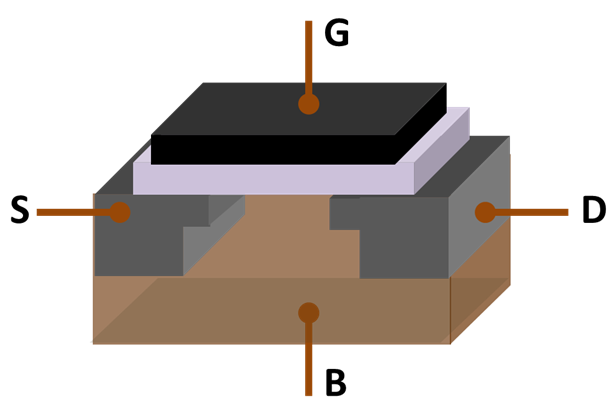
\includegraphics[width=\textwidth]{gfx/MOSFET_Structure.png}
            \column{0.7\textwidth}
            \begin{itemize}
                \item Solitamente implementati attraverso MOSFET\footnote{MOSFET: Metal Oxide Semiconductor Field Effect Transistor}
                \item 2 stati definiti (0, 1)
                \item Può trovarsi in uno tra gli stati 0 o 1
            \end{itemize}
        \end{columns}
    \end{frame}

    \begin{frame}{Qubit}
        \begin{columns}
            \column{0.3\textwidth}
            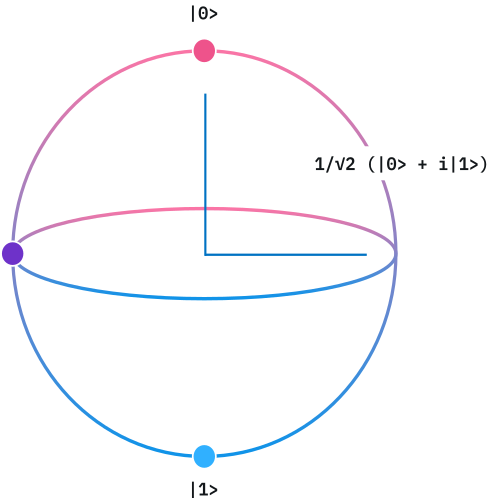
\includegraphics[width=\textwidth]{gfx/qubit_ibm.png}
            \column{0.7\textwidth}
            \begin{itemize}
                \item Può essere $\ket{0}$ o $\ket{1}$
                \item Può anche essere $\ket{0}$ e $\ket{1}$ contemporaneamente (sovrapposizione quantistica)
            \end{itemize}
        \end{columns}
    \end{frame}

    \begin{frame}{Qubit}
        Matematicamente, la sovrapposizione di un qubit è espressa come
        \begin{equation*}
            \ket{\psi} = \alpha \ket{0} + \beta \ket{1} = \begin{matrix}
                0 \\ 1
            \end{matrix}\begin{pmatrix}
                \alpha \\ \beta
            \end{pmatrix}
            , \quad \alpha, \beta \in \mathbb{C}, 
        \end{equation*}
        dove $\alpha$ e $\beta$ sono chimate ampiezze di probabilità. 
        
        L'ultima espressione è chiamata vettore di probabilità. 
    \end{frame}

    \begin{frame}{Sfera di Bloch}
        \begin{columns}
            \column{.3\textwidth}
            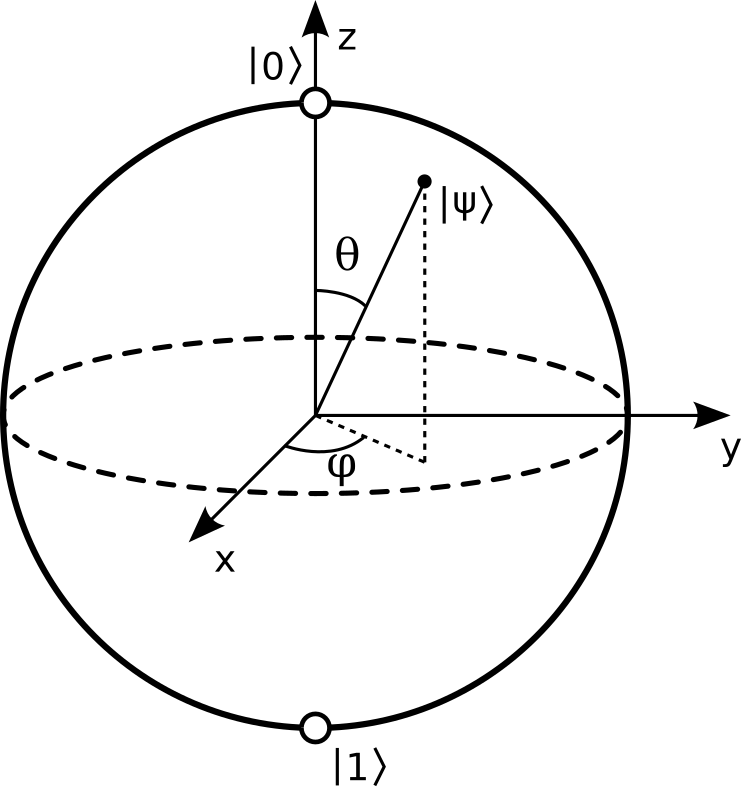
\includegraphics[width=\textwidth]{gfx/Bloch_sphere.png}
            \column{.7\textwidth}
            Un qubit si può visualizzare su una 2-sfera parametrizzando $\alpha$ e $\beta$ in coordinate polari
            \begin{equation*}
                \ket{\psi} = \cos \frac{\theta}{2} \ket{0} + e^{i\varphi}\sin \frac{\theta}{2} \ket{1},
            \end{equation*}
            dove $0\leq\theta\leq\pi$ e $0\leq\varphi<2\pi$
        \end{columns}
    \end{frame}

    \begin{frame}{Registro di 2 qubit}
        Un computer quantistico con $n$ qubit ha $2^n$ ampiezze di probabilità. 

        Lo stato di un registro a più qubit è rappresentato dal prodotto tensore dello stato dei singoli qubit. 

        \begin{equation*}
            \ket{00} = \ket{0} \otimes \ket{0}
        \end{equation*}
        \begin{equation*}
            \ket{\psi} = c_0 \ket{00} + c_1 \ket{01} + c_2 \ket{10} + c_3 \ket{11} = 
            \begin{matrix}
                00 \\ 01 \\ 10 \\ 11
            \end{matrix} \begin{pmatrix}
                c_0 \\ c_1 \\ c_2 \\ c_3
            \end{pmatrix}
        \end{equation*}  
    \end{frame}

    \begin{frame}{Registro di $n$ qubit}
        Un computer quantistico con $n$ qubit ha $2^n$ ampiezze di probabilità. 

        Lo stato di un registro a più qubit è rappresentato dal prodotto tensore dello stato dei singoli qubit. 

        \begin{equation*}
            \ket{00\ldots00} = \ket{0} \otimes \ket{0} \otimes \ldots \otimes \ket{0} \otimes \ket{0}
        \end{equation*}
        \begin{equation*}
            \begin{split}
                \ket{\psi} &= c_0 \ket{00\ldots00} + c_1 \ket{00\ldots01} + \ldots + c_{n-2} \ket{11\ldots10} + \\ 
                &+ c_{n-1} \ket{11\ldots11} = \begin{matrix}
                00\ldots00 \\ 00\ldots01 \\ \vdots \\ 11\ldots10 \\ 11\ldots11
            \end{matrix} \begin{pmatrix}
                c_0 \\ c_1 \\ \vdots \\ c_{n-2} \\ c_{n-1}
            \end{pmatrix}
            \end{split}
        \end{equation*}
    \end{frame}

    \begin{frame}{Porte logiche quantistiche}
        Per manipolare $n$ qubit esistono apposite porte logiche quantistiche, 
        che sono operatori rappresentabili come matrici $2^n\times2^n$. 
        \begin{columns}
            \column{.3\textwidth}
            \begin{figure}[]
                \centering
                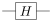
\includegraphics[width=\textwidth]{gfx/Hadamard_gate}
                \caption{Hadamard}
                \label{}
            \end{figure}
            \column{.3\textwidth}
            \begin{figure}[]
                \centering
                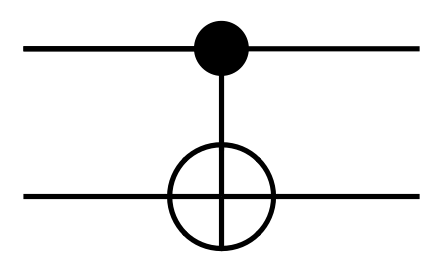
\includegraphics[width=\textwidth]{gfx/CNOT_gate}                
                \caption{CNOT}
                \label{}
            \end{figure}
            \column{.3\textwidth}
            \begin{figure}[]
                \centering
                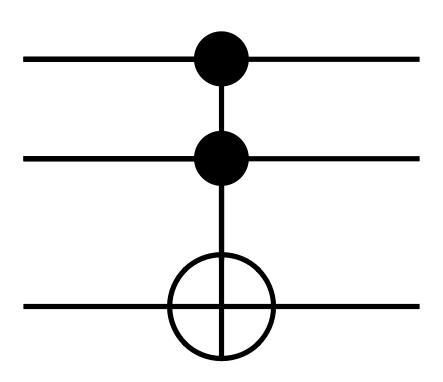
\includegraphics[width=\textwidth]{gfx/Toffoli_gate}                
                \caption{Toffoli}
                \label{}
            \end{figure}
        \end{columns}
    \end{frame}

    \begin{frame}{Punti di forza dei quantum computer}
        \begin{columns}
            \column{.45\textwidth}
            \begin{tabular}{p{.15\textwidth}p{.8\textwidth}}
                \# di qubit & RAM classica richiesta \\ \hline
                5 & 256 byte \\ 
                25 & 2 gigabyte \\ 
                50 & 8000 terabyte \\ 
                275 & numero di atomi nell'universo osservabile 
            \end{tabular}
            \column{.45\textwidth}
            Le $n$ ampiezze di probabilità possono essere usate per memorizzare quantità enormi di informazioni. 

            Possiamo inoltre creare e lavorare su più copie in parallelo degli stessi dati. 
        \end{columns}
    \end{frame}

    \begin{frame}{Stato dell'arte}
        \begin{columns}
            \column{.3\textwidth}
            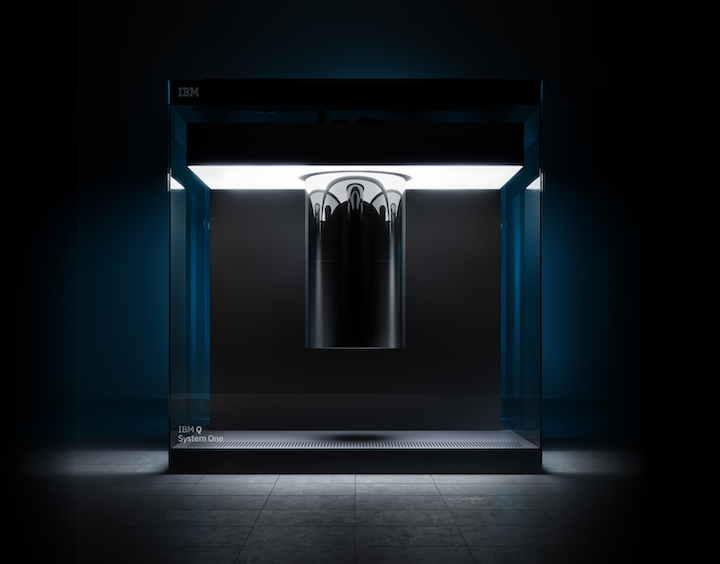
\includegraphics[width=\textwidth]{gfx/ibm_q_system_one.png}
            \column{.7\textwidth}
            L'IBM Q System One è il primo computer quantistico a circuiti commerciale al mondo, 
            introdotto dall'IBM nel gennaio 2019. L'IBM Q System One possiede 20 qubit. 
        \end{columns}
    \end{frame}

    \section{Metodi}

    \begin{frame}{IBM Q Experience}
        \begin{columns}
            \column{.3\textwidth}
            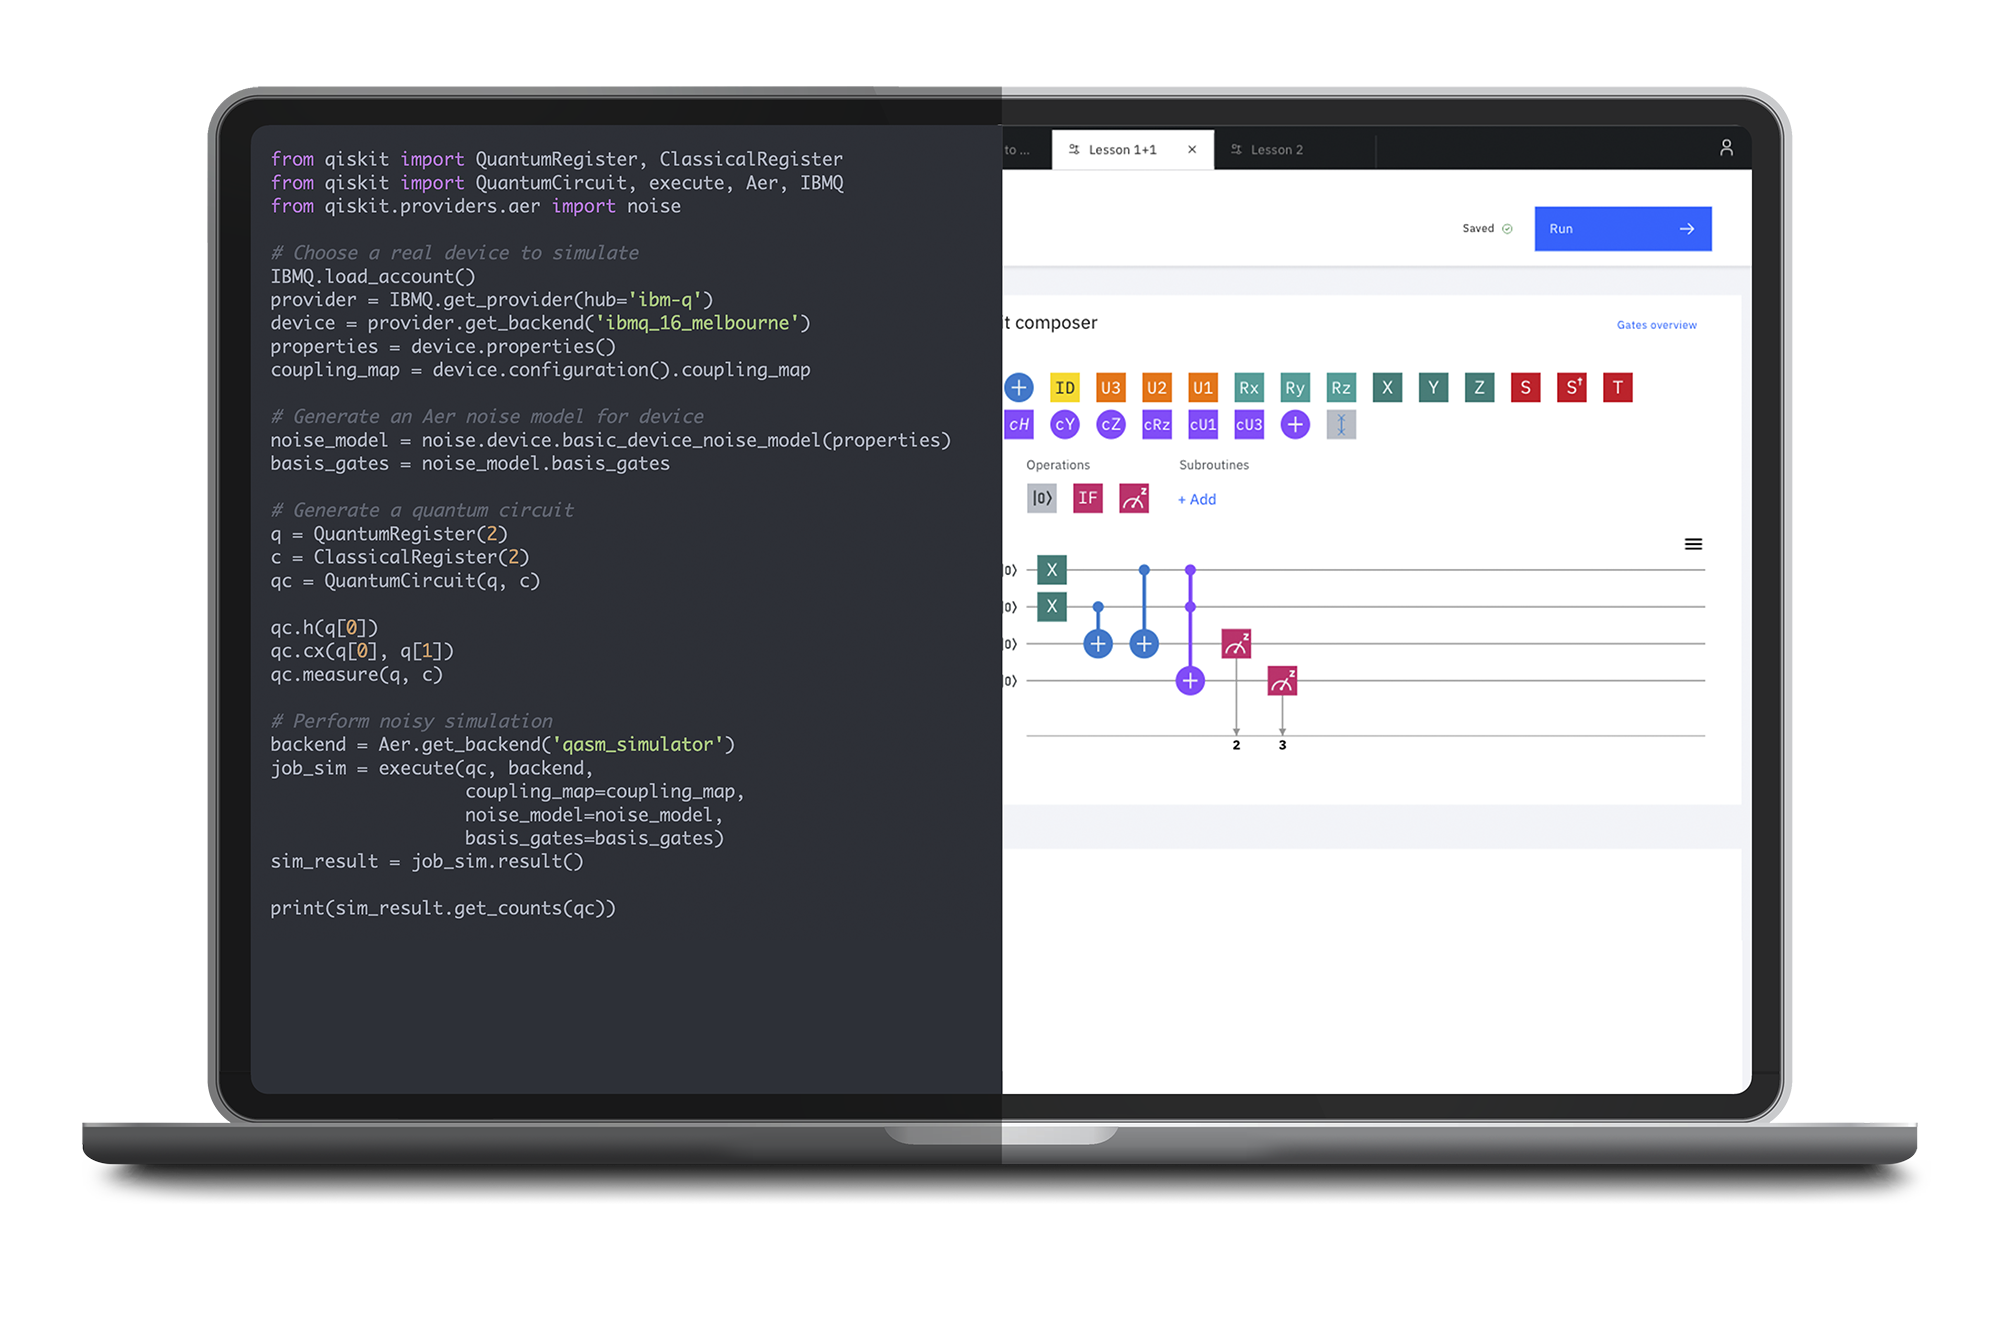
\includegraphics[width=\textwidth]{gfx/laptop_strumenti.png}
            \column{.7\textwidth}
            L'IBM Q Experience è un'interfaccia per interagire con le risorse di quantum computing dell'IBM
            \begin{itemize}
                \item accessibile al pubblico
                \item permette simulazioni con e senza rumore
                \item fino a 14 qubit superconduttivi
                \item fino a 32 qubit simulati
            \end{itemize}
        \end{columns}
    \end{frame}

    \begin{frame}{Qiskit}
        \begin{columns}
            \column{.3\textwidth}
            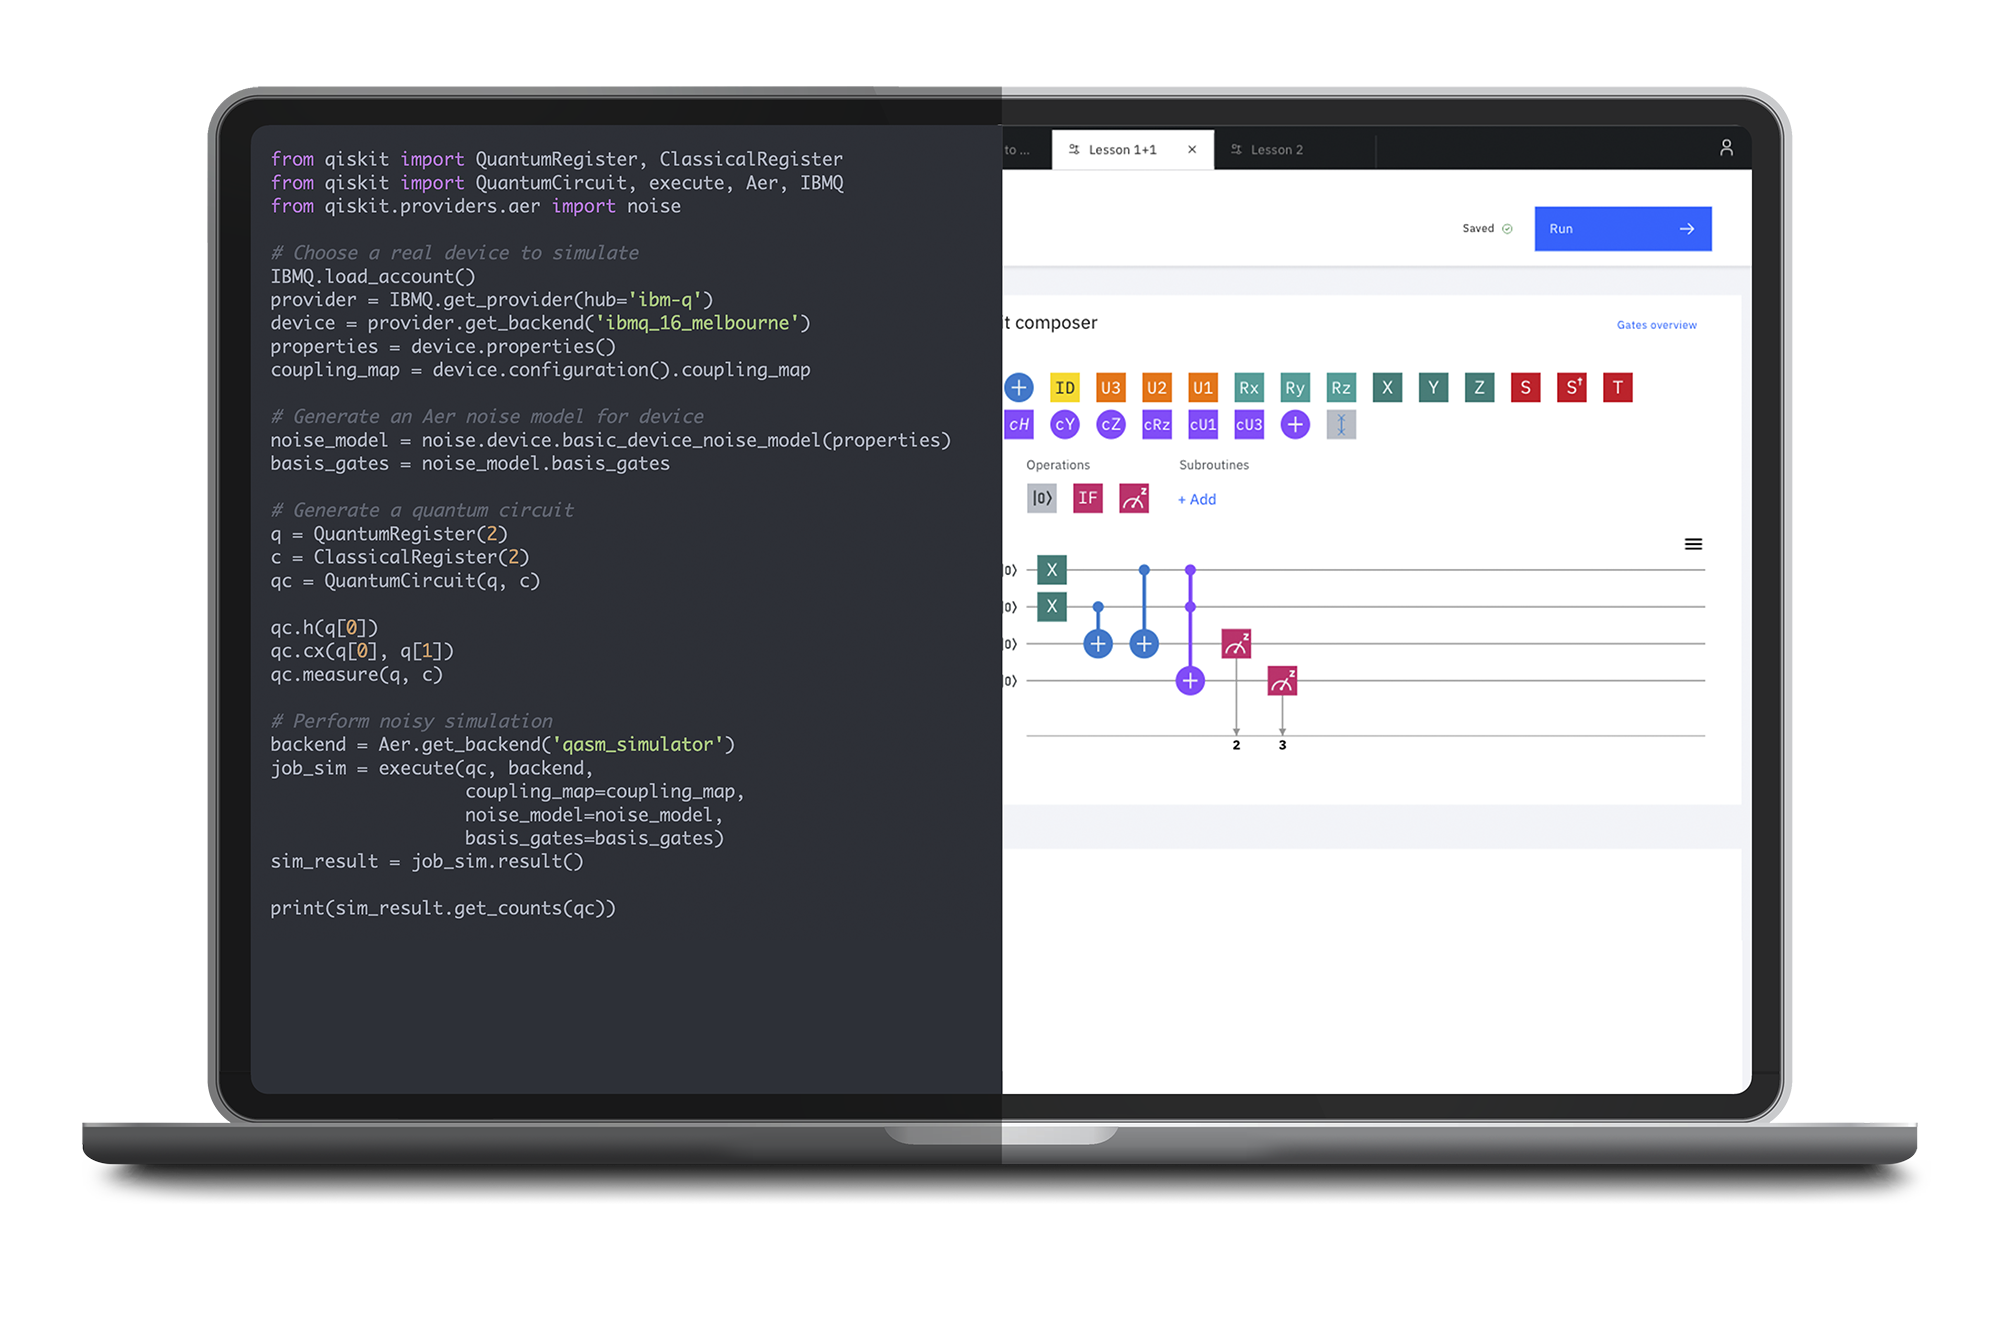
\includegraphics[width=\textwidth]{gfx/laptop_strumenti.png}
            \column{.7\textwidth}
            Struttura open source di sviluppo software per quantum computing, permette di 
            \begin{itemize}
                \item progettare circuiti quantistici
                \item simularli sul proprio computer personale
                \item inviare ordini di esecuzione su harware quantistico reale
                \item visualizzare i risultati
            \end{itemize}
        \end{columns}
    \end{frame}

    \section{Quantum machine learning}

    \begin{frame}{Codificare dati classici nelle ampiezze}
        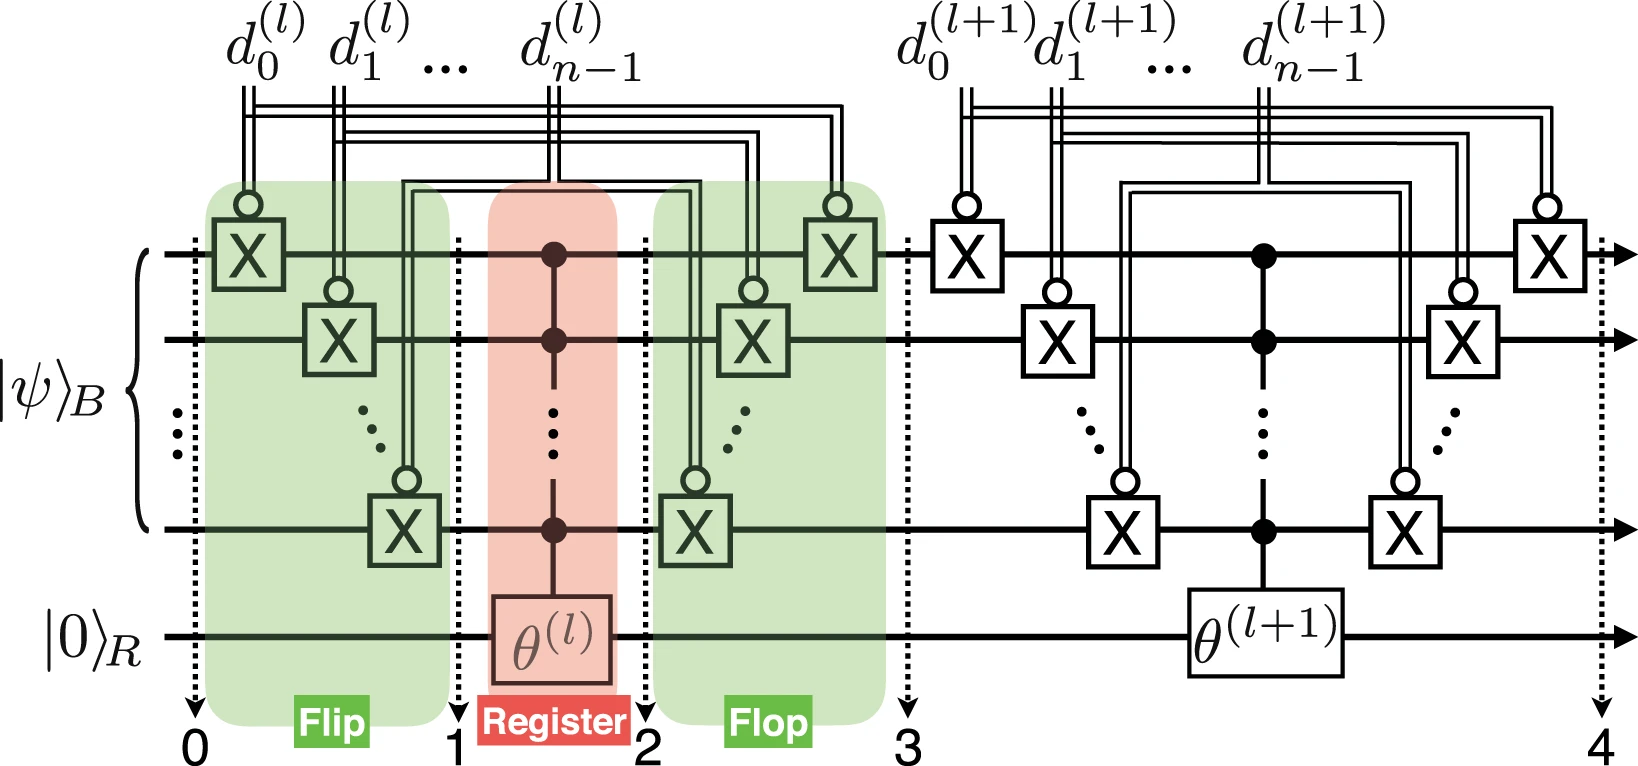
\includegraphics[width=\textwidth]{gfx/qram.png}
        Per codificare dati classici nelle ampiezze di probabilità è stata usata la tecnica di costruzione 
        di stati flip-flop QRAM, come proposto da Petruccione et al.
    \end{frame}

    \begin{frame}{FF-QRAM}
        La FF-QRAM è usata per memorizzare un QDB inizializzato in maniera arbitraria. 

        L'operazione QRAM sui qubit sovrappone un insieme di dati classici 
        $D = \left\{ \left( \vec{d}^{(l)}, b_l \right) \Big| 0 \leq l < M \right\}$ come
        \begin{equation*} \label{eq:qram}
            \text{QRAM}(D) \sum_j \psi_j \ket{j}_B \ket{0}_R \equiv 
            \sum_l \psi_l \ket{\vec{d}^{(l)}}_B \ket{b_l}_R,
        \end{equation*}
        dove $\vec{d}^{(l)}$ rappresenta un indirizzo di memoria con 
        $n$ bit di informazione 
        e $b_l$ è l'attributo ad esso associato. 
    \end{frame}

    \begin{frame}{Algoritmo KNN quantistico}
        Stato quantistico iniziale

		\begin{equation*}
			\ket{\psi_0} = \frac{1}{\sqrt{2M}} \sum_{m=1}^M 
			(\ket{0}\ket{\psi_x}+\ket{1}\ket{\psi_{t^m}})\ket{c^m}\ket{m}
		\end{equation*}

		Calcolo della distanza con interferenza quantistica

		\begin{equation*}
			\ket{\psi_1} = \frac{1}{2\sqrt{M}}\sum_{m=1}^M 
			\Big( \ket{0}(\ket{\psi_x}+\ket{\psi_{t^m}}) + \ket{1}(\ket{\psi_x}-\ket{\psi_{t^m}}) \Big) \ket{c^m}\ket{m}
		\end{equation*}
	
		Misura condizionale

		\begin{equation*}
			\ket{\psi_2} = \frac{1}{2\sqrt{M}} \sum_{m=1}^M \sum_{i=1}^N
			(x_i+t_i^m)\ket{0}\ket{i}\ket{c^m}\ket{m}
		\end{equation*}
    \end{frame}

    \begin{frame}{Algoritmo KNN quantistico}
        Probabilità di misurare una data classe

		\begin{equation*}
			\text{P}(\ket{c^m} = \ket{s}) = \sum_{m|c^m=s} 
			1 - \frac{1}{4M} |x-t^m|^2
		\end{equation*}

		Classificazione

		\begin{equation*}
			c = \begin{cases}
			0 \quad \text{se}\, \text{P}(\ket{c^0})\, \text{maggiore} \\
			1 \quad \text{se}\, \text{P}(\ket{c^1})\, \text{maggiore} \\
			\text{etc}\ldots
		\end{cases}
		\end{equation*}
    \end{frame}

    \section{Implementazione}

    \begin{frame}{Preparazione dei dati}
        \begin{figure}[h]
            \centering
            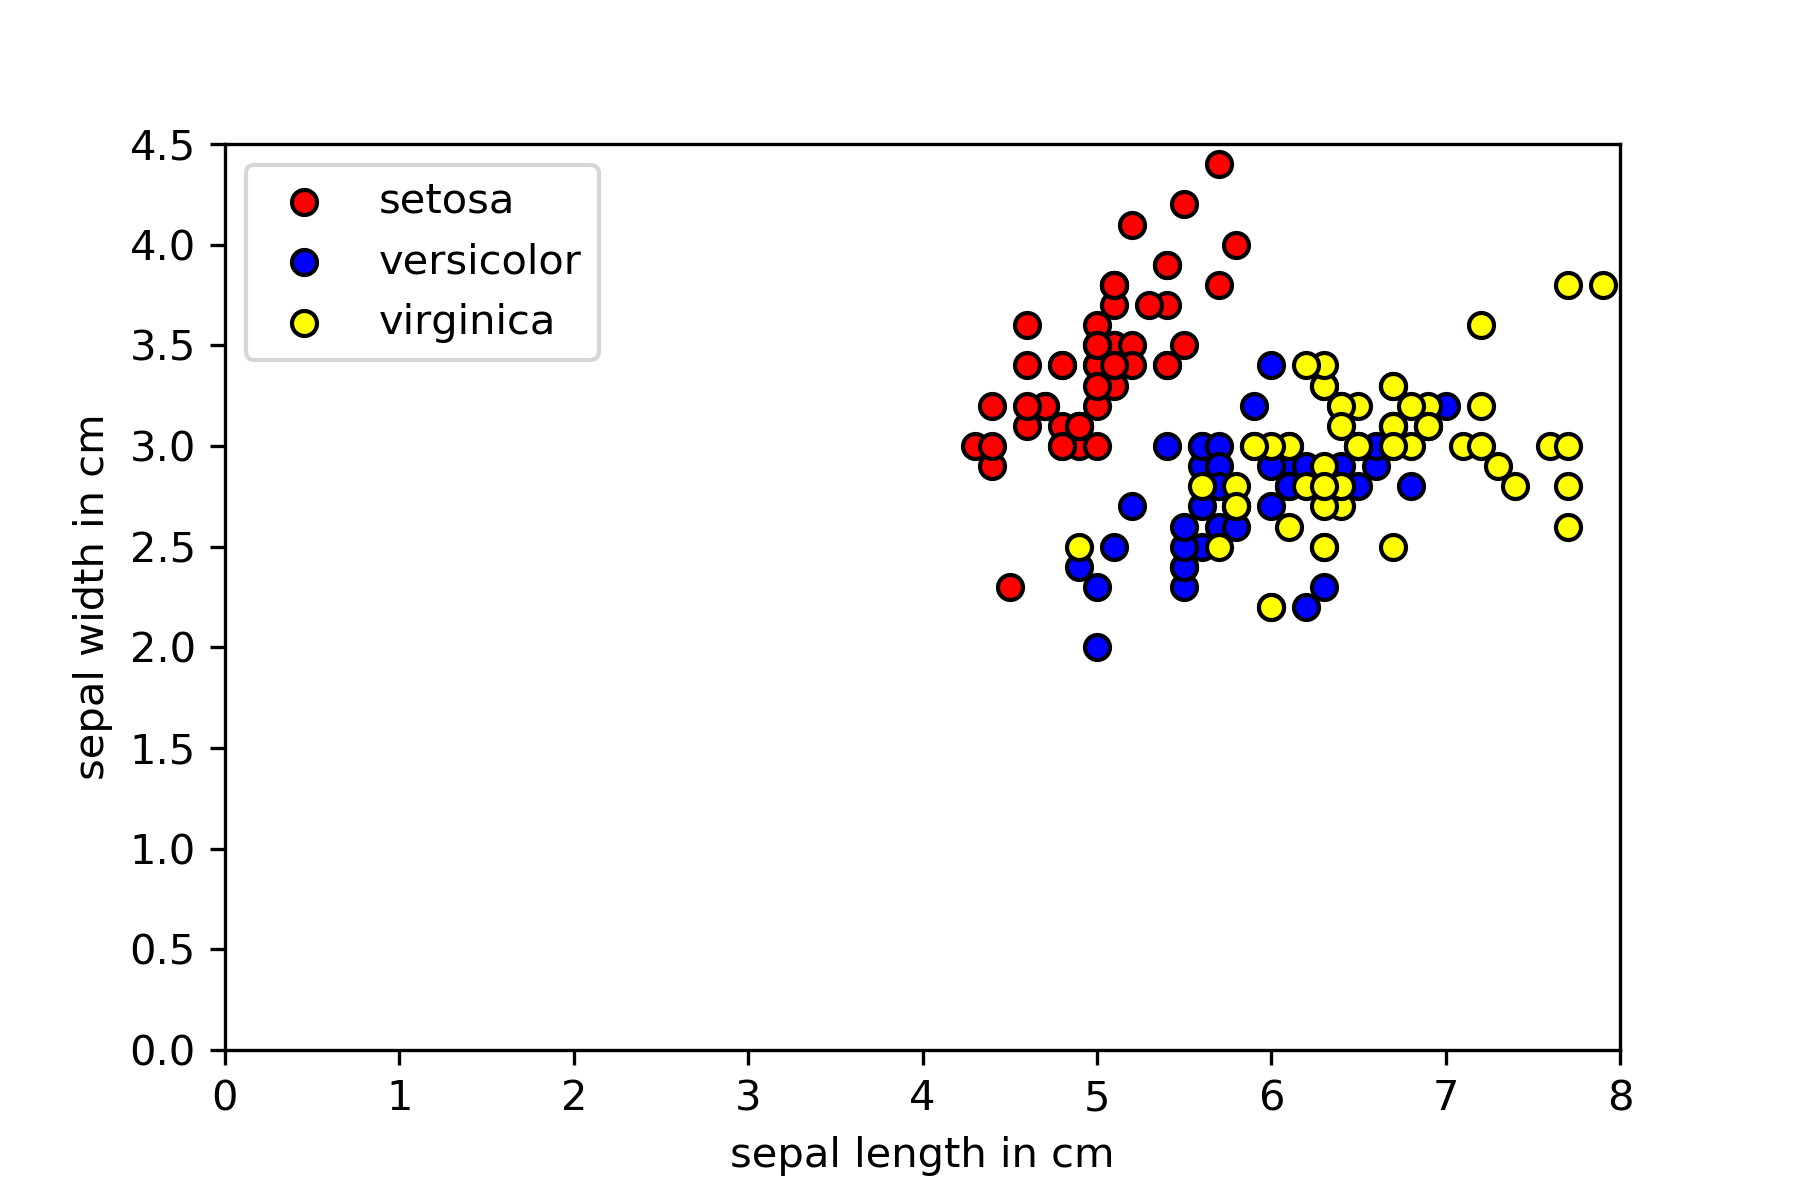
\includegraphics[width=.8\textwidth]{gfx/iris/iris4features}
            \caption{Data set Iris}
            \label{}
        \end{figure}
    \end{frame}

    \begin{frame}{Preparazione dei dati}
        \begin{figure}[h]
            \centering
            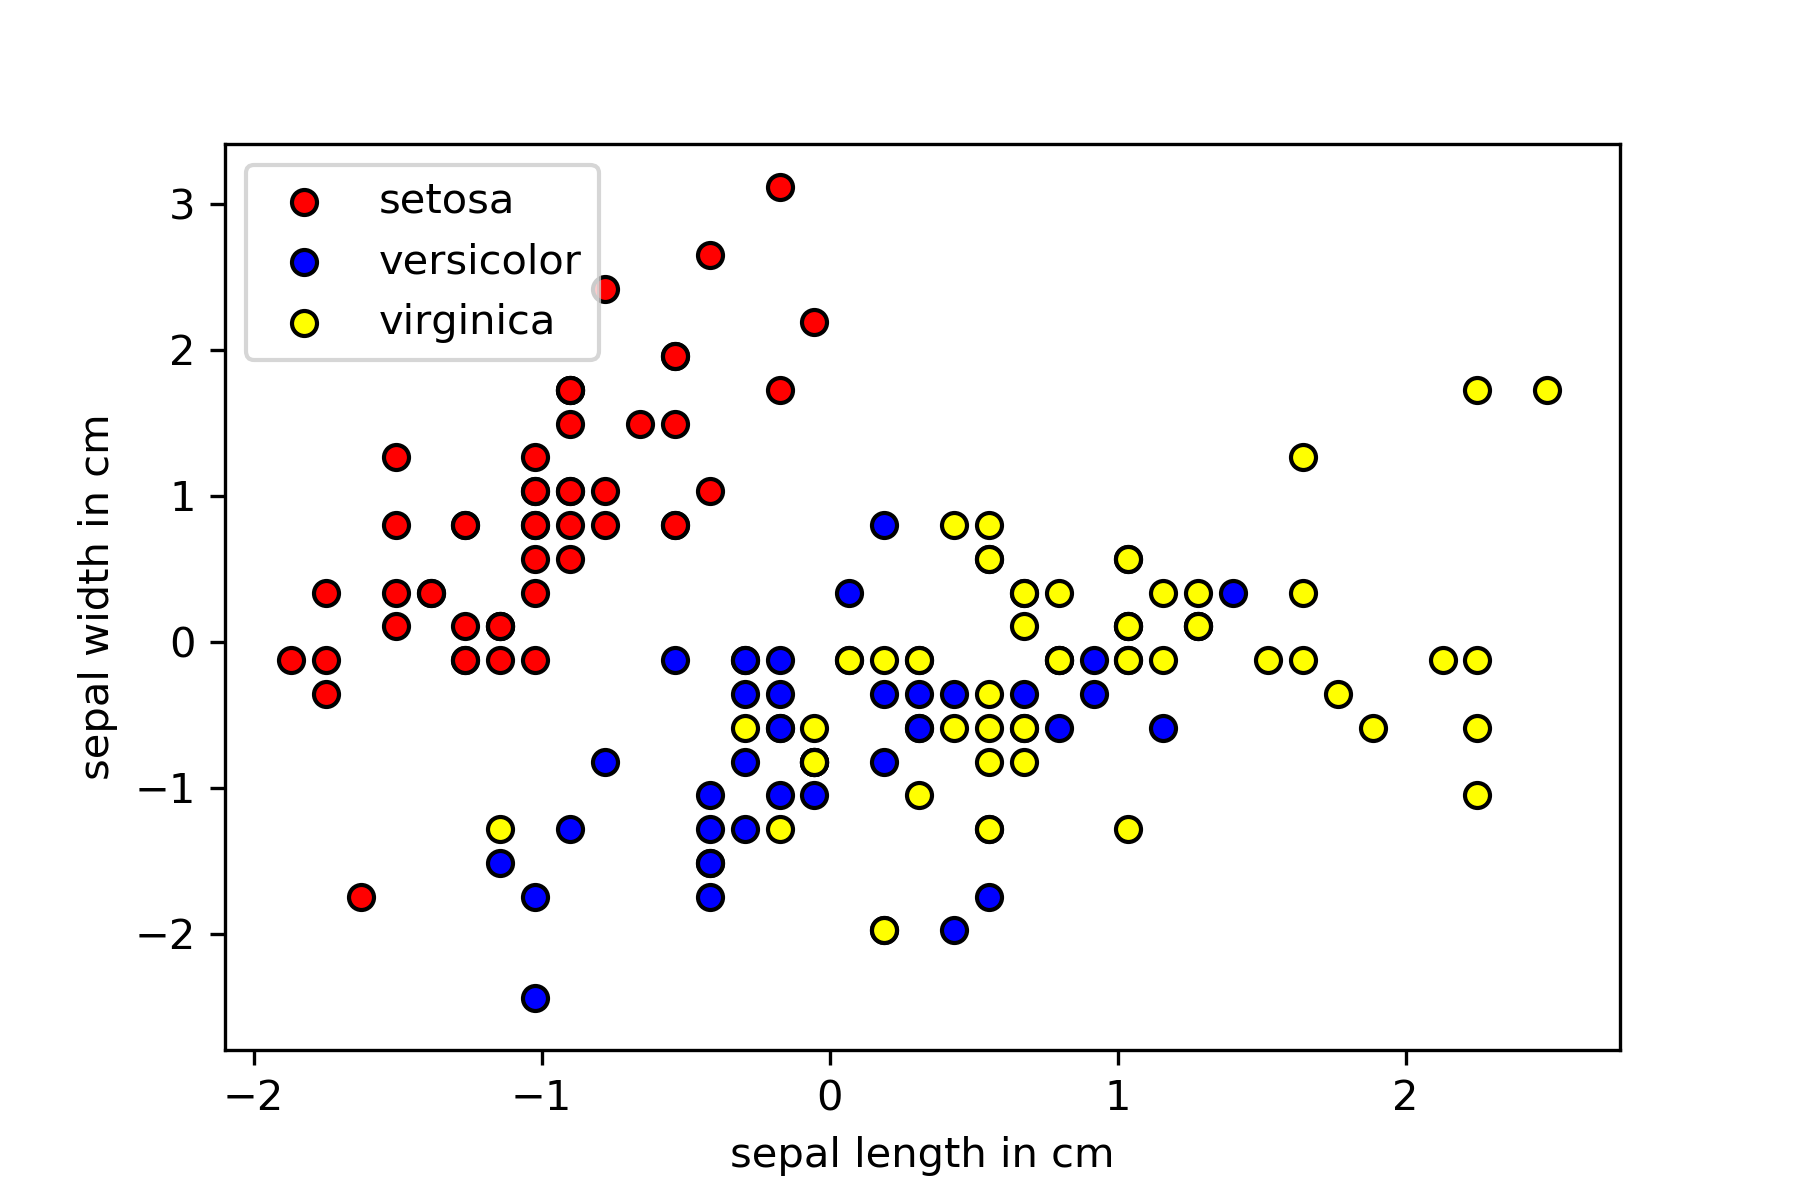
\includegraphics[width=.8\textwidth]{gfx/iris/irisscaled}
            \caption{Data set Iris standardizzato}
            \label{}
        \end{figure}
    \end{frame}

    \begin{frame}{Preparazione dei dati}
        \begin{figure}[h]
            \centering
            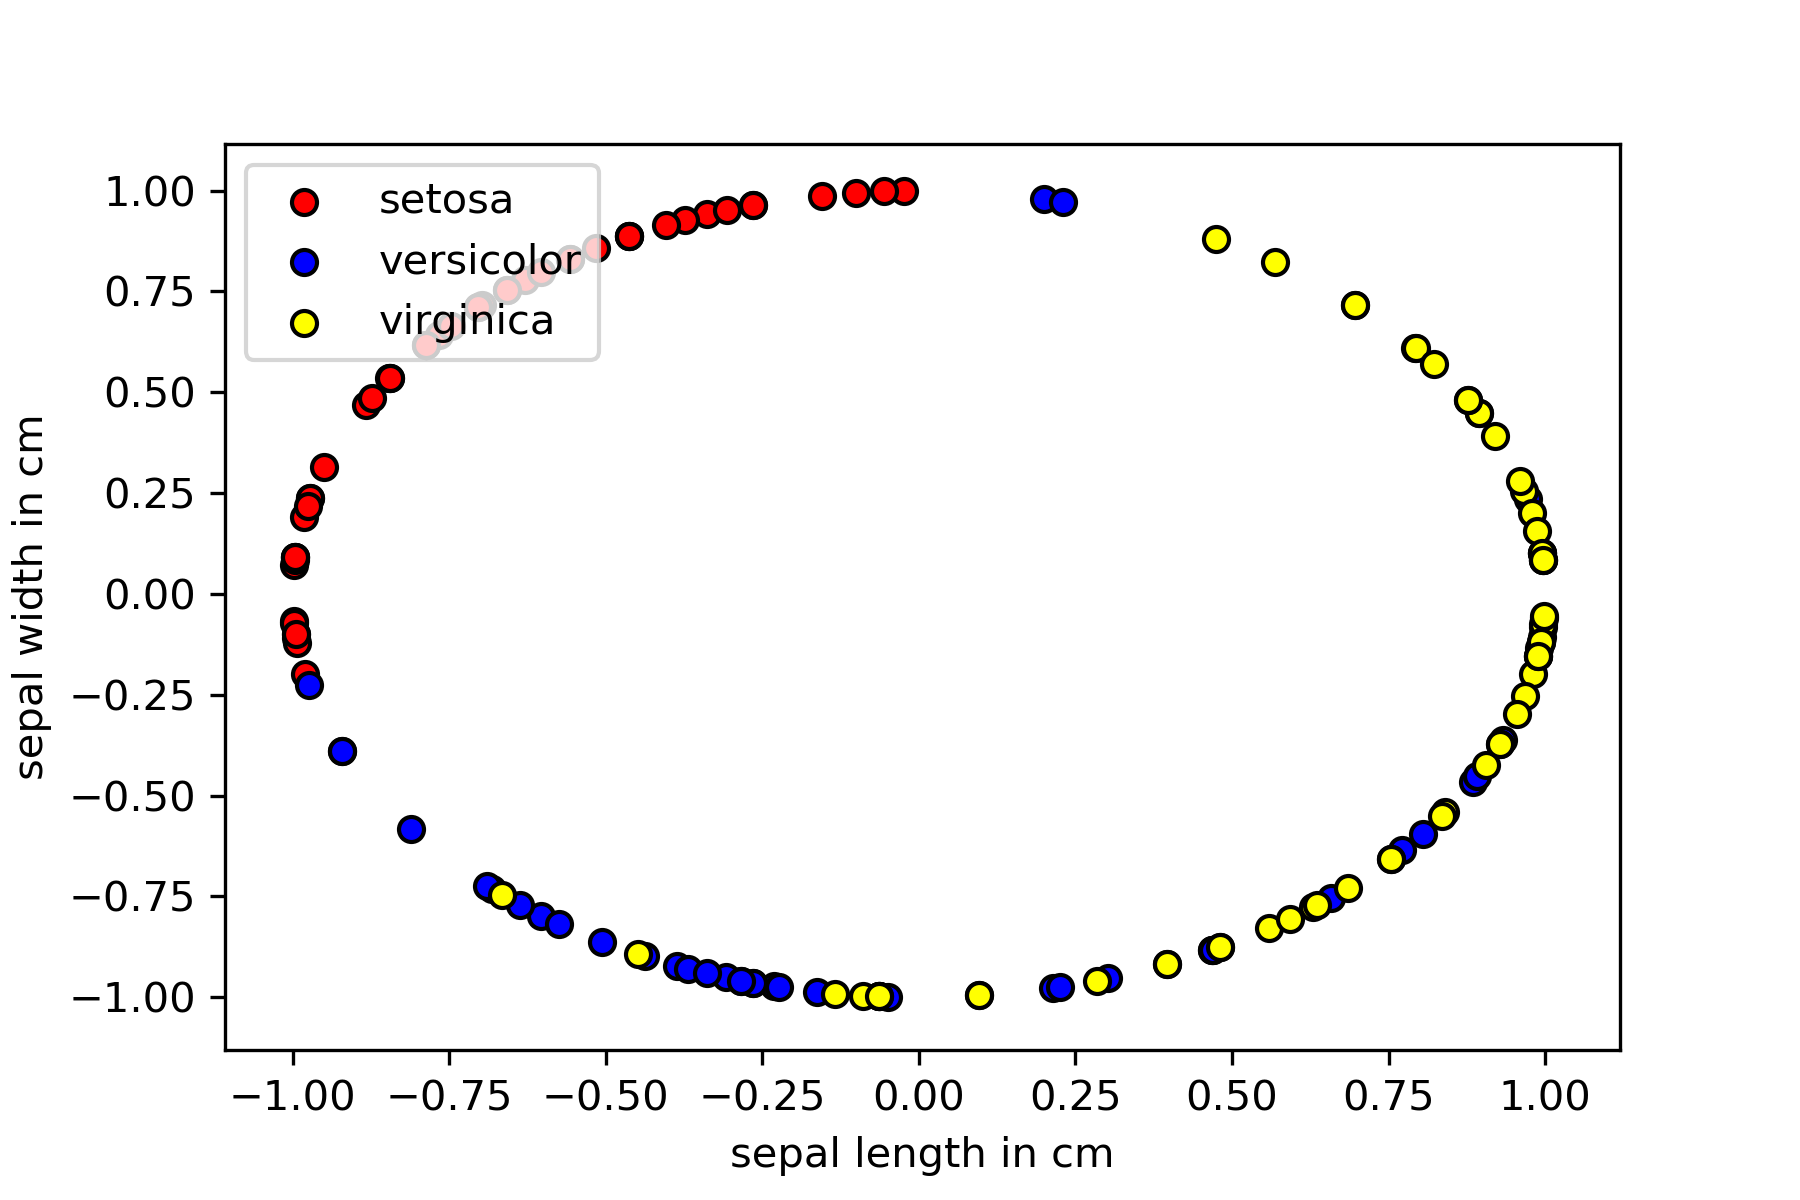
\includegraphics[width=.8\textwidth]{gfx/iris/irisnormalized}
            \caption{Data set Iris normalizzato (2 caratteristiche)}
            \label{}
        \end{figure}
    \end{frame}

    \begin{frame}{Preparazione dei dati}
        \begin{figure}[h]
            \centering
            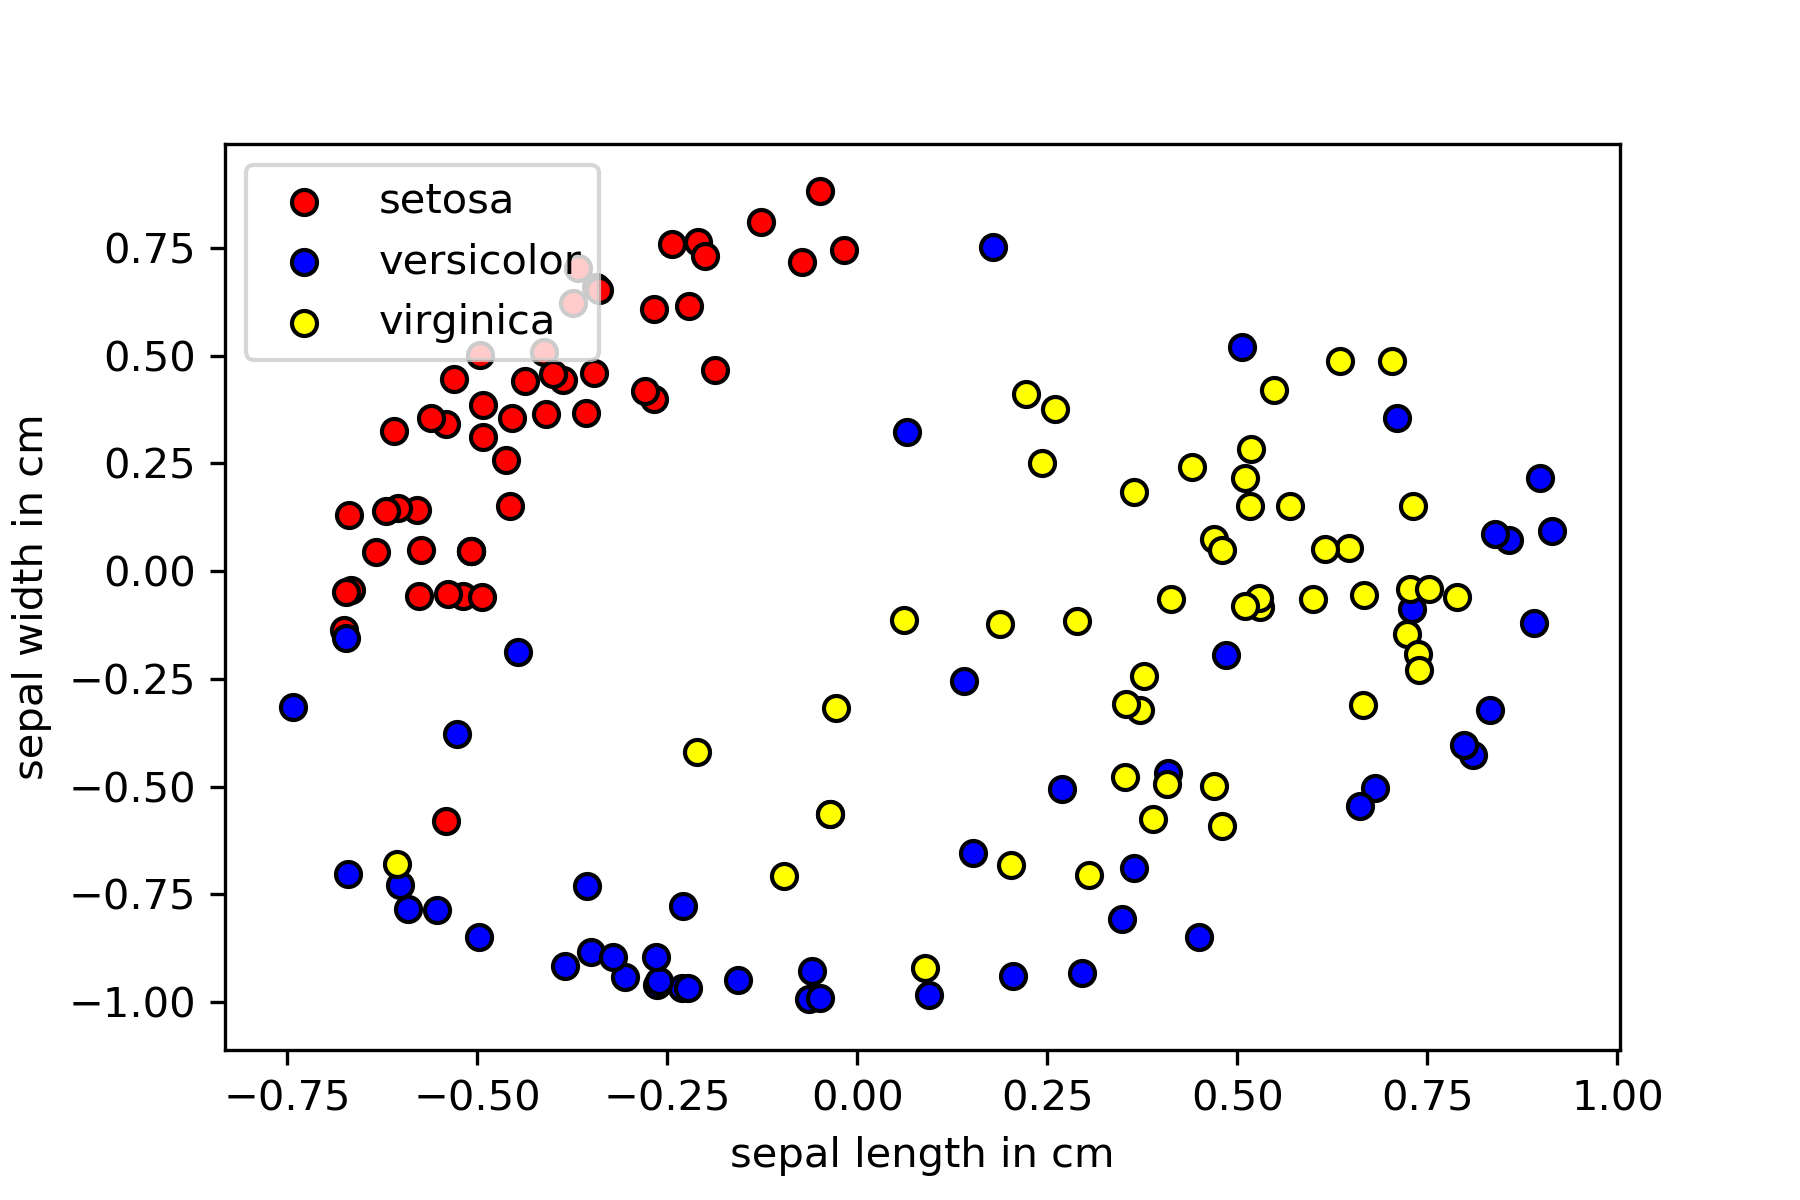
\includegraphics[width=.8\textwidth]{gfx/iris/iris4normalized}
            \caption{Data set Iris normalizzato (4 caratteristiche)}
            \label{}
        \end{figure}
    \end{frame}

    \begin{frame}{Il circuito quantistico}
        Il circuito quantistico per un classificatore binario è il seguente
        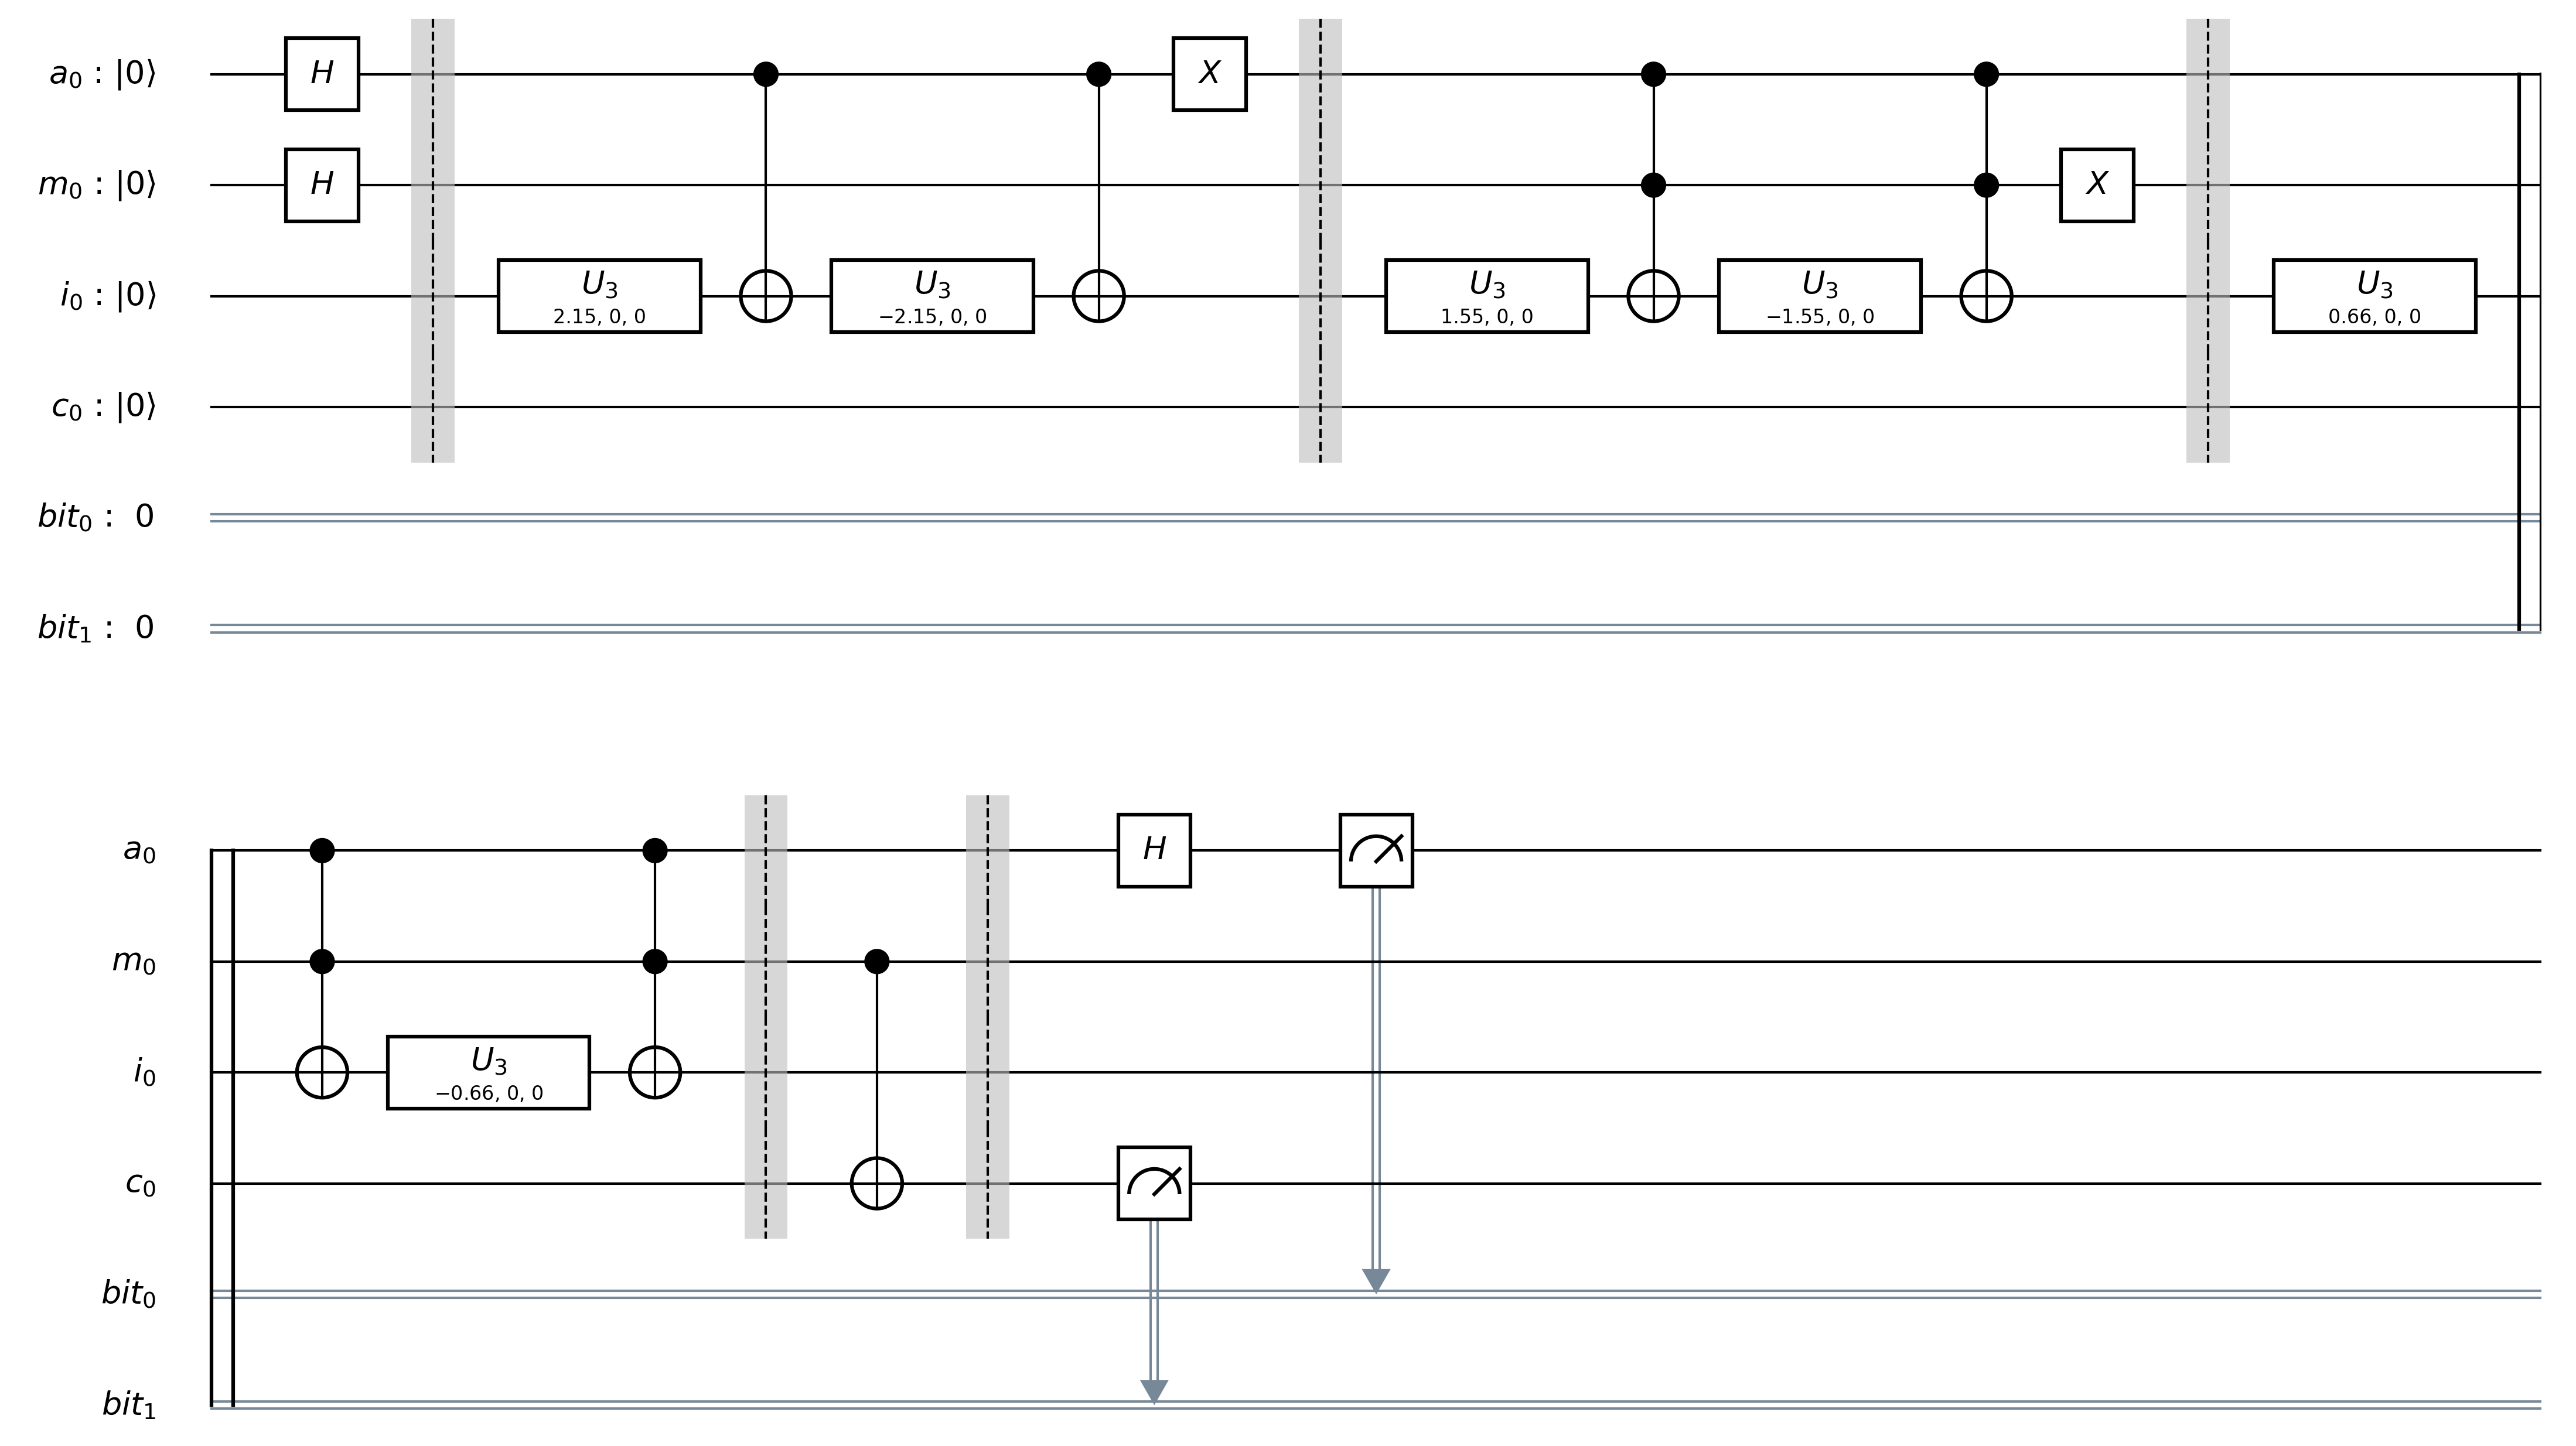
\includegraphics[width=\textwidth]{gfx/base_circuit_crop}
        Per il classificatore multiclasse il disegno è più complicato. 
    \end{frame}

    \section{Risultati}

    \begin{frame}{Classificazione binaria}
        Classificazione setosa vs. versicolor dal data set Iris
        \begin{columns}
            \column{.5\textwidth}
            \begin{figure}[h]
                \centering
                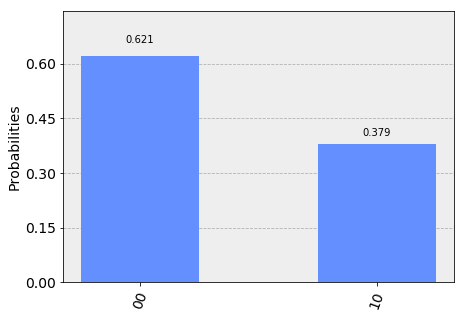
\includegraphics[width=\textwidth]{gfx/iris/iris2SetosaVersicolorResult.png}
                \caption{Simulazione su setosa}
                \label{fig:simulazione.setosa}
            \end{figure}
            \column{.5\textwidth}
            \begin{figure}[h]
                \centering
                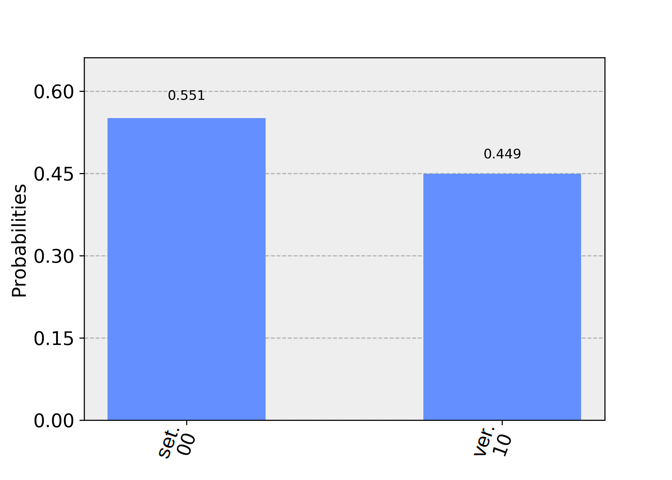
\includegraphics[width=\textwidth]{gfx/misura_setosa_sperimentale.png}
                \caption{Esecuzione reale su setosa}
                \label{fig:esecuzione.setosa}
            \end{figure}
        \end{columns}
    \end{frame}

    \begin{frame}{Classificazione multiclasse}
        Classificazione setosa vs. versicolor vs. virginica dal data set Iris
        \begin{columns}
            \column{.5\textwidth}
            \begin{figure}[h]
                \centering
                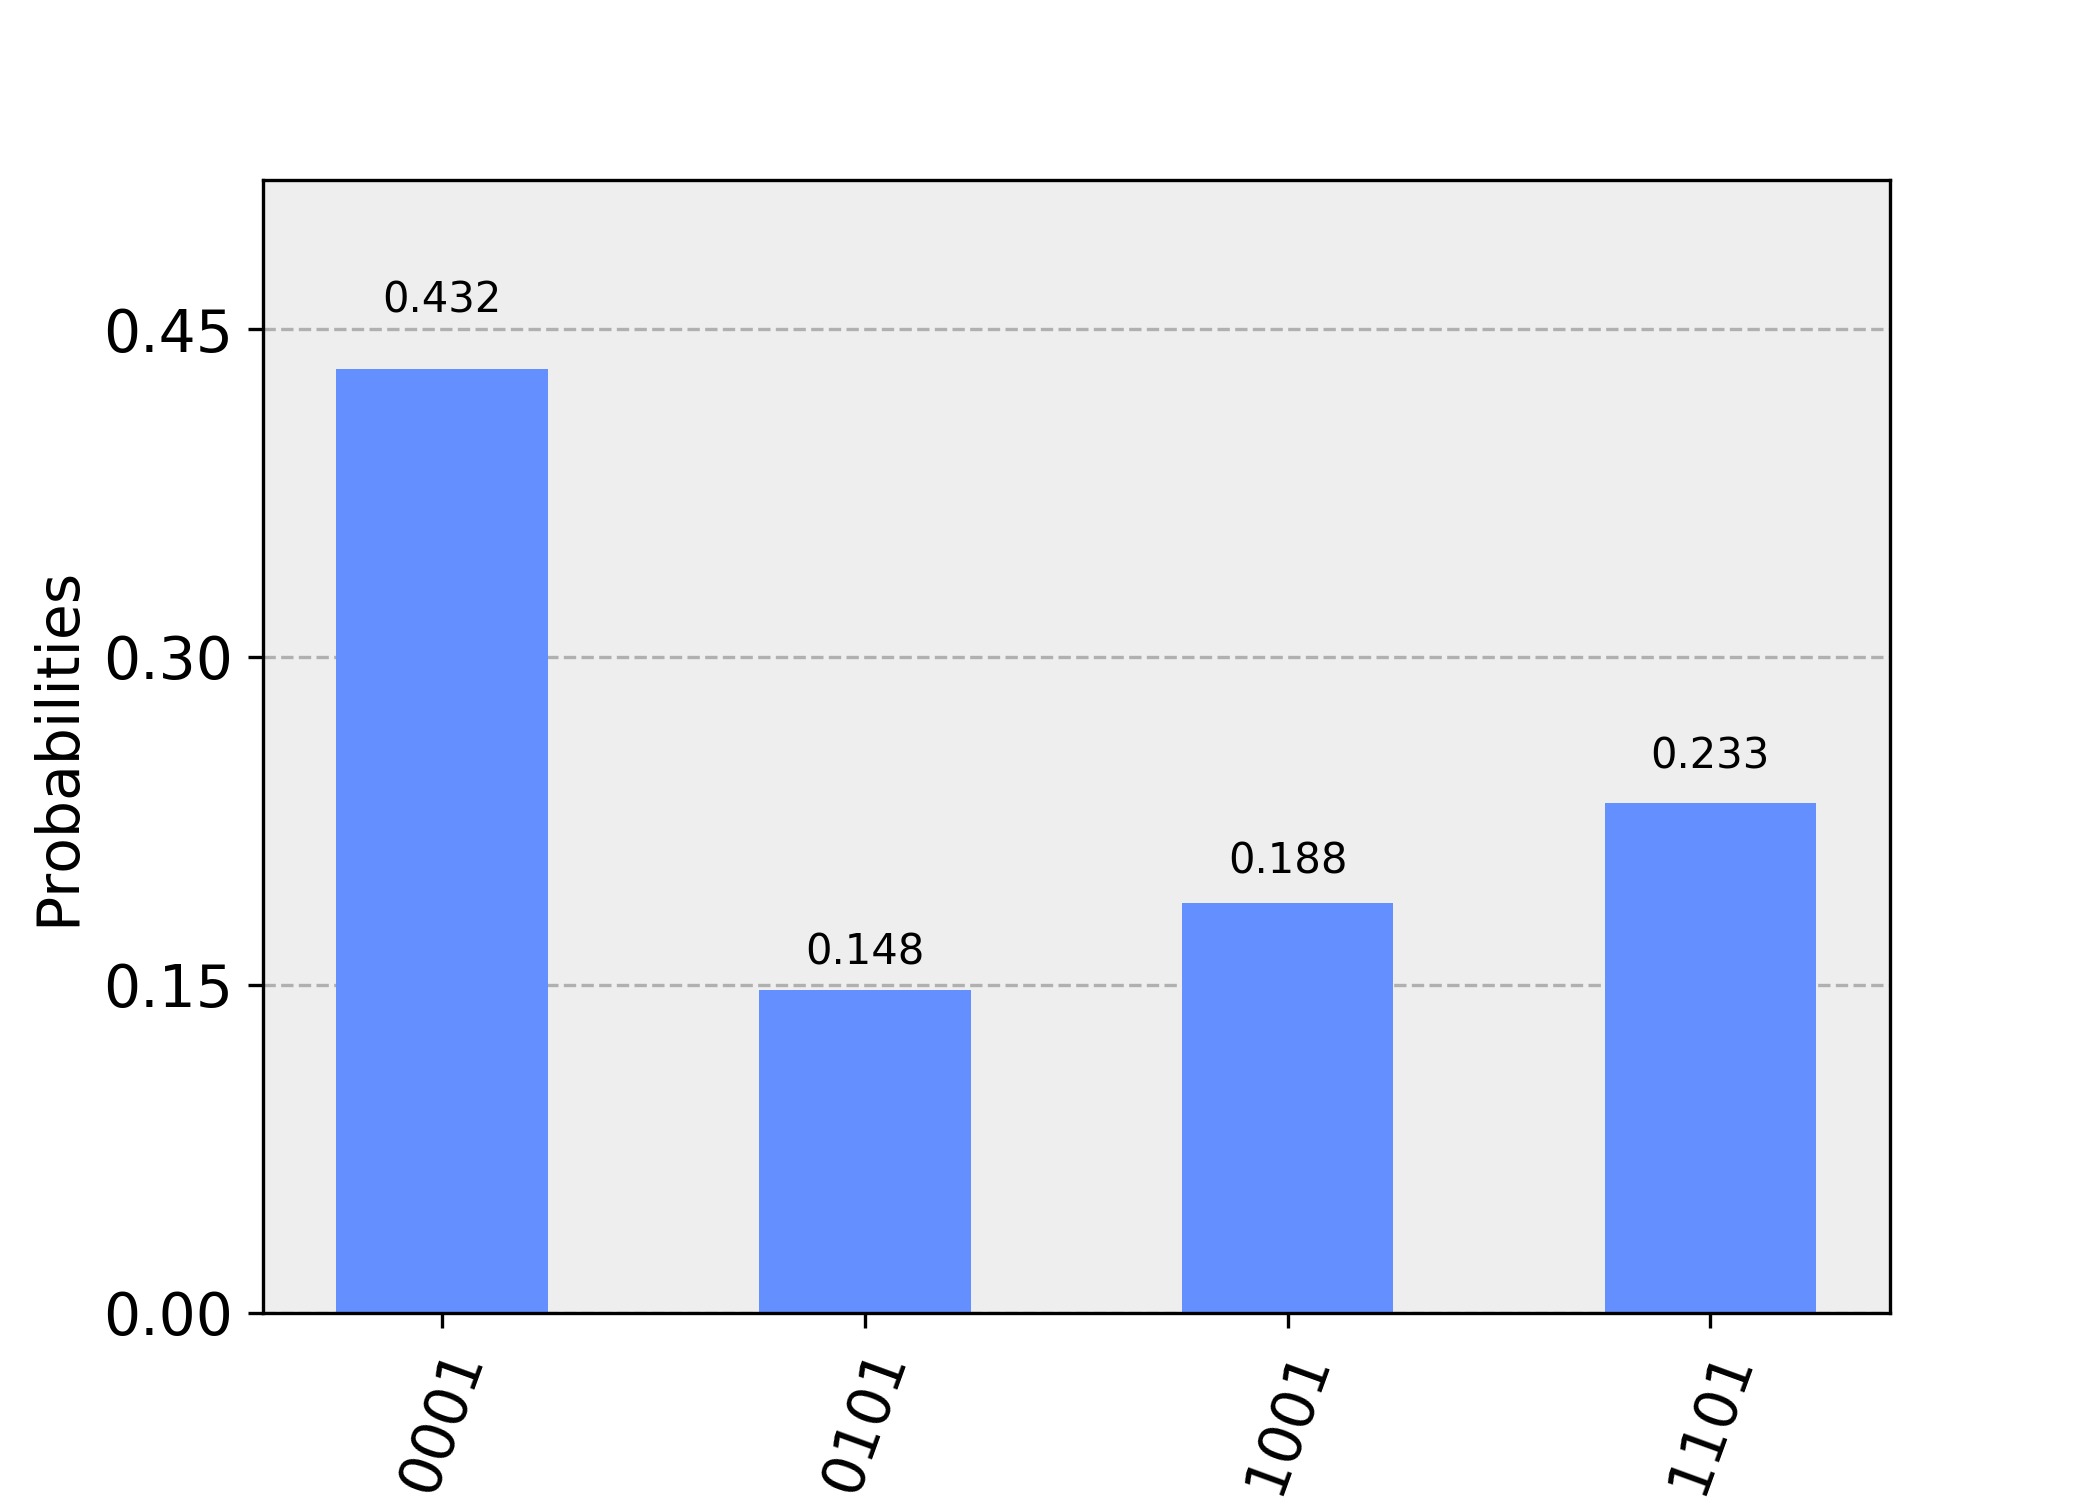
\includegraphics[width=\textwidth]{gfx/setosa_simulato_multiclasse.png}
                \caption{Simulazione su setosa}
                \label{fig:simulazione.multi.setosa}
            \end{figure}
            \column{.5\textwidth}
            \begin{figure}[h]
                \centering
                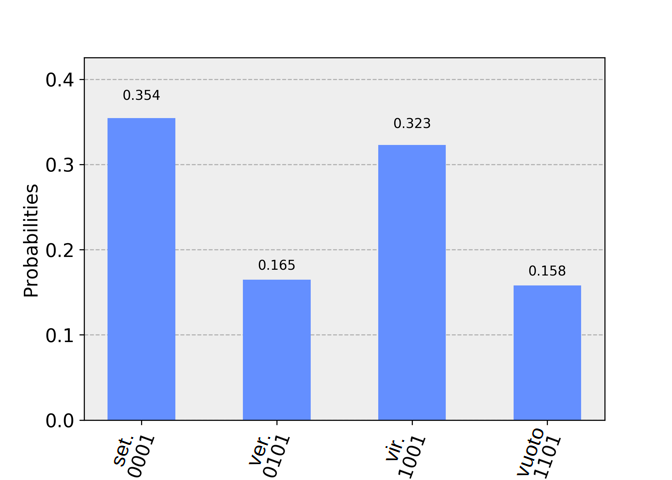
\includegraphics[width=\textwidth]{gfx/setosa_reale_20190913:1716.png}
                \caption{Esecuzione reale su setosa}
                \label{fig:esecuzione.multi.setosa}
            \end{figure}
        \end{columns}
    \end{frame}

    \section{Conclusione}

    \begin{frame}{Riassunto}
        \begin{itemize}
            \item L'elaborazione quantistica è nella frontiera dei supercomputer e ha il potenziale di accelerare gli algoritmi di machine learning classico
            \item È stata riprodotta un'implementazione di algoritmo KNN quantistico di classificazione binaria su hardware di piccola scala
            \item Se ne è esteso il funzionamento in modo da renderlo multiclasse
            \item Si sono effettuati test su hardware quantistico di media scala
        \end{itemize}
    \end{frame}

    \begin{frame}{Prospettive}
        \begin{itemize}
            \item Far girare gli algoritmi su computer con maggiori risorse, sia in termini di numero di qubit che di tempi di decoerenza
            \item A tal proposito, sarebbe interessante l'esecuzione sul computer a 20 qubit annunciato quest'anno
            \item Si attende lo sviluppo di corrispettivi quantistici per algoritmi di IA più complessi
        \end{itemize}
    \end{frame}

    \begin{frame}[focus]
        Domande?
    \end{frame}

    \appendix

    \begin{frame}{Algoritmo per classificatore binario}
        \begin{block}{Inizializzazione dei registri quantistici}
            a = QuantumRegister(1, 'a') \\
            m = QuantumRegister(1, 'm') \\
            i = QuantumRegister(1, 'i') \\
            c = QuantumRegister(1, 'c') \\
            b = ClassicalRegister(2, 'bit') \\
            circuit = QuantumCircuit(a, m, i, c, b)
        \end{block}

        \begin{block}{Sovrapposizione degli stati}
            circuit.h(a) \\
            circuit.h(m)
        \end{block}

        \begin{block}{Codifica del vettore d'input}
            circuit.cry(x0, a[0], i[0]) \\
            circuit.x(a) \# entanglement dell'ancilla con 0
        \end{block}
    \end{frame}

    \begin{frame}{Algoritmo per classificatore binario}
        \begin{block}{Codifica dei vettori di training}
            circuit.mcry(t0, a[:] + m[:], i[0], None) \\
            circuit.x(m) \# entanglement di m con 0 \\
            circuit.mcry(t1, a[:] + m[:], i[0], None) \\
            circuit.cx(m, c) \# entanglement della classe 1 con m 1 \\
        \end{block}

        \begin{block}{Interferenza degli stati}
            circuit.h(a)
        \end{block}
        
        \begin{block}{Operazione di misura}
            circuit.measure(a, b[0]) \\
            circuit.measure(c, b[1]) \\
        \end{block}
        \# circuit.draw(output='mpl')
    \end{frame}

    \begin{frame}{Algoritmo per classificatore multiclasse}
        \begin{block}{Inizializzazione dei registri quantistici}
            a = QuantumRegister(1, 'a') \# knn ancilla \\
            m = QuantumRegister(2, 'm') \# training vector index \\
            i = QuantumRegister(2, 'i') \# feature index \\
            r = QuantumRegister(1, 'r') \# rotation qubit \\
            q = QuantumRegister(5, 'q') \# qram ancilla \\
            c = QuantumRegister(2, 'c') \# class \\
            b = ClassicalRegister(4, 'bit') \\
            circuit = QuantumCircuit(a, m, i, r, q, c, b)
        \end{block}

        \begin{block}{Sovrapposizione degli stati}
            circuit.h(a) \\
            circuit.h(m) \\
            circuit.h(i) \\
            circuit.h(c)
        \end{block}
    \end{frame}

    \begin{frame}{Algoritmo per classificatore multiclasse}
        \begin{block}{Codifica dei vettori}
            \# circuit.cry(theta, control, target) \\
            \# circuit.mcry(theta, controls, target, ancillae) \\

            \# >> Encode the input vector >> \\

            encodeVector(circuit, inputVirginica, i, a[:] + i[:], r[0], q) \\ 

            circuit.x(a) \# entanglement dell'ancilla con 0 \\

            \# >> Encode the training vectors >> \\

            buildTrainingState(trainingArray) \\
        \end{block}
        \begin{block}{Interferenza e misura}
            circuit.measure(r, b[0]) \\
            circuit.h(a) \\
            circuit.measure(a, b[1]) \\
            circuit.measure(c[0], b[2]) \\
            circuit.measure(c[1], b[3])
        \end{block}
    \end{frame}

    \begin{frame}{Algoritmo per classificatore multiclasse}
        \begin{block}{Definizione dei costruttori}
            def encodeTraining(circuit, data, i, controls, rotationQ, ancillaQ, c, m): \\
            \# Header \\
            encodeClass(circuit, c) \\
            encodeIndex(circuit,m) \\
            \# Encoder \\
            encodeVector(circuit, data, i, controls, rotationQ, ancillaQ) \\
            \# Footer \\
            encodeClass(circuit, c) \\
            encodeIndex(circuit, m)
        \end{block}
    \end{frame}

    \begin{frame}{Algoritmo per classificatore multiclasse}
        \begin{block}{Definizione del codificatore}
            def encodeVector(circ, data, i, controls, rotationQ, ancillaQ): \\
            \# |00>\\
            circuit.x(i)\\
            circuit.mcry(data[0], controls, rotationQ, ancillaQ)\\
            circuit.x(i)\\
            \# |01>\\
            circuit.x(i[1])\\
            circuit.mcry(data[1], controls, rotationQ, ancillaQ)\\
            circuit.x(i[1])\\
            \# |10>\\
            circuit.x(i[0])\\
            circuit.mcry(data[2], controls, rotationQ, ancillaQ)\\
            circuit.x(i[0])\\
            \# |11>\\
            circuit.mcry(data[3], controls, rotationQ, ancillaQ)
        \end{block}
    \end{frame}
\end{document}
